%% Satellite Navigation (SpringerOpen)

\documentclass[pdflatex,sn-basic]{sn-jnl}

%%%% Standard packages
\usepackage{graphicx}
\usepackage{multirow}
\usepackage{amsmath,amssymb,amsfonts}
\usepackage{amsthm}
\usepackage{mathrsfs}
\usepackage[title]{appendix}
\usepackage{xcolor}
\usepackage{textcomp}
\usepackage{booktabs}
\usepackage{bm}
\usepackage{siunitx}
\usepackage{xspace}
\usepackage{url}

%% Theorem styles
\theoremstyle{thmstyleone}
\newtheorem{theorem}{Theorem}
\newtheorem{proposition}[theorem]{Proposition}
\theoremstyle{thmstyletwo}
\newtheorem{example}{Example}
\newtheorem{remark}{Remark}
\theoremstyle{thmstylethree}
\newtheorem{definition}{Definition}

%% Custom commands
\newcommand{\eg}{\textit{e.g.}\xspace}
\newcommand{\ie}{\textit{i.e.}\xspace}
\newcommand{\etal}{\textit{et al.}\xspace}
\newcommand{\cnzero}{$C/N_0$\xspace}
\newcommand{\linf}{\ell_\infty}
\newcommand{\eps}{\varepsilon}

\raggedbottom

\begin{document}

\title[Adversarial Vulnerability of GNSS Spoofing Detectors]{Adversarial Vulnerability of Machine Learning GNSS Spoofing Detectors to Transmitted Spoofing Signals}

\author*[1]{\fnm{Joel Segun} \sur{Ojerinde}}\email{joelojerinde@buaa.edu.cn}
\author*[1]{\fnm{Wasiu Akande} \sur{Ahmed}}\email{ahmedwasiu24@buaa.edu.cn}
\author[2]{\fnm{Akinyinka Olukunle} \sur{Akande}}

\affil*[1]{\orgdiv{Regional Centre for Space Science and Technology Education in Asia and the Pacific (RCSSTEAP), Hangzhou International Innovation Institute}, \orgname{Beihang University}, \orgaddress{\city{Hangzhou 311115}, \country{China}}}

\affil[2]{\orgname{Federal University of Technology}, \orgaddress{\city{Owerri}, \country{Nigeria}}}

\abstract{A spoofer broadcasts counterfeit Global Navigation Satellite System (GNSS)
signals so that a victim receiver computes a false position or time. Detectors trained by machine learning are increasingly
proposed for this threat, but are evaluated against fixed corpora of recorded attacks that
do not respond to the detector under test. This paper evaluates fourteen detectors, eight
classical and six deep, under attacks that are radio signals selected by an adversary. A
counterfeit GPS L1 C/A waveform is synthesised at sample level, summed with authentic
recordings from the Texas Spoofing Test Battery and tracked by the FGI-GSRx software
receiver, so that the observables each detector reads are produced by receiver processing
of a transmittable signal. The adversary sets counterfeit power, code pull-off rate and
carrier frequency and phase, with no knowledge of the detector and no query access. The
generator is validated by reproducing data set ds7, whose construction is published. All
detectors are placed at a common operating point flagging 95 percent of spoofed samples on
clean validation data, and evaluated against 126 settings satisfying the published
conditions for receiver takeover. Clean performance predicts resistance poorly and the two
orderings are close to inverted: the random forest attains the highest clean $F_1$ score of
0.833 and the lowest false alarm rate of 0.337, yet is evaded by 55 of the 126 attacks.
Detectors evading none flag 46 to 74 percent of authentic data. One evaded attack drives
the receiver clock at 48.89 nanoseconds per second against a commanded 48.87.}

\keywords{GNSS spoofing, Spoofing detection, Machine learning, Software defined
receiver, Resilient PNT, Receiver in the loop testing}

\maketitle

\section{Introduction}
\label{sec:intro}

\subsection{GNSS spoofing and its detection}

A Global Navigation Satellite System (GNSS) supplies a receiver with its position, its
velocity and its time. Power grids use that time to synchronise, financial systems use it
to stamp transactions, and aircraft and autonomous platforms use the position to navigate
\citep{kaplan2005understanding}. The civil signal that carries this service is public and
unencrypted, and its structure is fully specified in open documents, so a transmitter of
modest cost can generate a waveform with the same modulation, the same spreading code and
the same message format as a genuine satellite. A spoofer is such a transmitter. It emits
counterfeit satellite signals with the intention that a victim receiver tracks them in
preference to the authentic ones and reports a position or a time of the spoofer's
choosing. The threat is not hypothetical: a spoofer has steered a yacht off its intended
course through the ship's navigation system \citep{bhatti2017hostile}, and a spoofer has
captured an airborne platform in flight \citep{kerns2014uav}.

Spoofing differs from jamming in a way that determines how it must be handled. A jammer
denies the service, and the receiver observes that it has lost lock. A spoofer leaves the
receiver operating nominally while the solution it reports is wrong, so the receiver holds
no internal evidence that anything has occurred and the attack must be identified while it
is in progress \citep{psiaki2016gnss}. Capturing a receiver that is already tracking
authentic signals is correspondingly more demanding than simply transmitting at higher
power. The published procedure proceeds in three stages: the counterfeit is first aligned
with the authentic signal in code phase, carrier phase and Doppler frequency, so that the
victim's correlator sees a single undistorted peak; its power is then raised slightly above
the authentic power, typically by a few decibels; and only then is the counterfeit dragged
away from the authentic signal, carrying the tracking loops with it and moving the reported
position or time \citep{psiaki2016gnss,kerns2014uav}. A counterfeit that omits the
alignment stage does not capture the receiver at all, and acts only as interference. The
consequence is that the attacker's freedom is bounded: not every combination of transmitter
settings takes over a receiver, and an evaluation that ignores this distinction credits a
detector for rejecting transmissions that would never have succeeded.

Classical anti-spoofing tests monitor quantities the receiver computes in the course of
tracking a satellite. Representative examples are the carrier-to-noise density ratio, which
reflects received signal strength; the shape of the correlation function, which distorts
when a second copy of the same code is present; and the agreement between code and carrier
measurements of a single satellite \citep{akos2012gnss,psiaki2016gnss}. Each such test
identifies one physical signature of an attack, which makes it interpretable and also makes
it evadable: a spoofer that holds the named quantity within its nominal range passes the
test, and the set of tests a receiver runs is public knowledge.

\subsection{Learned detectors and how they are evaluated}

The limitation of signature based tests has motivated detectors inferred from data. A
machine learning detector is a classifier trained on labelled epochs, some recorded while
the receiver tracked authentic signals and some recorded under spoofing, which learns which
joint configurations of receiver measurements indicate an attack. Because such a classifier
reads many measurements simultaneously, it can exploit dependencies that no single hand
written statistic encodes, and recent work reports high detection accuracy for both deep
architectures and classical classifiers applied to receiver observables
\citep{borhanidarian2024deep,li2025realtime,chen2025cgan}. Physics constrained networks
extend the approach towards attacks absent from the training data by imposing relations that
authentic signals must satisfy \citep{song2026generalized}.

The evaluation practice that accompanies this literature is uniform: a detector is scored
against a fixed collection of recorded or simulated attacks. Those attacks were selected
before the detector existed, by whoever assembled the corpus, and they do not respond to the
classifier under test. A spoofer does respond. It selects the counterfeit power, the rate at
which it drags the code away from the authentic code, and the frequency and phase of its
carrier, and each of those choices alters the measurements the victim receiver produces and
therefore alters what the detector reads. Detection accuracy obtained against a fixed corpus
describes the corpus. It does not, by itself, characterise behaviour against an adversary
that chooses what to transmit, and the two quantities need not coincide.

\subsection{Receiver in the loop evaluation of transmitted attacks}

This paper evaluates fourteen detectors under attacks that are radio signals and not
perturbations of a measurement table. A counterfeit GPS L1 C/A waveform is synthesised at
sample level, summed with authentic recorded samples from the Texas Spoofing Test Battery
\citep{humphreys2012texbat,humphreys2016texbatds78}, passed through a model of the receiver
front end, and tracked by the FGI-GSRx software receiver \citep{fgigsrx}, published by the
Finnish Geospatial Research Institute (FGI). The observables
each detector reads are those the receiver computes while tracking that sum.
Figure~\ref{fig:geometry} contrasts authentic operation with a spoofing attack, and
Figure~\ref{fig:pipeline} shows the evaluation chain.

% Figure source: figures_src/static/fig_spoofing_geometry.png (hand made)
\begin{figure*}[t]
\centering
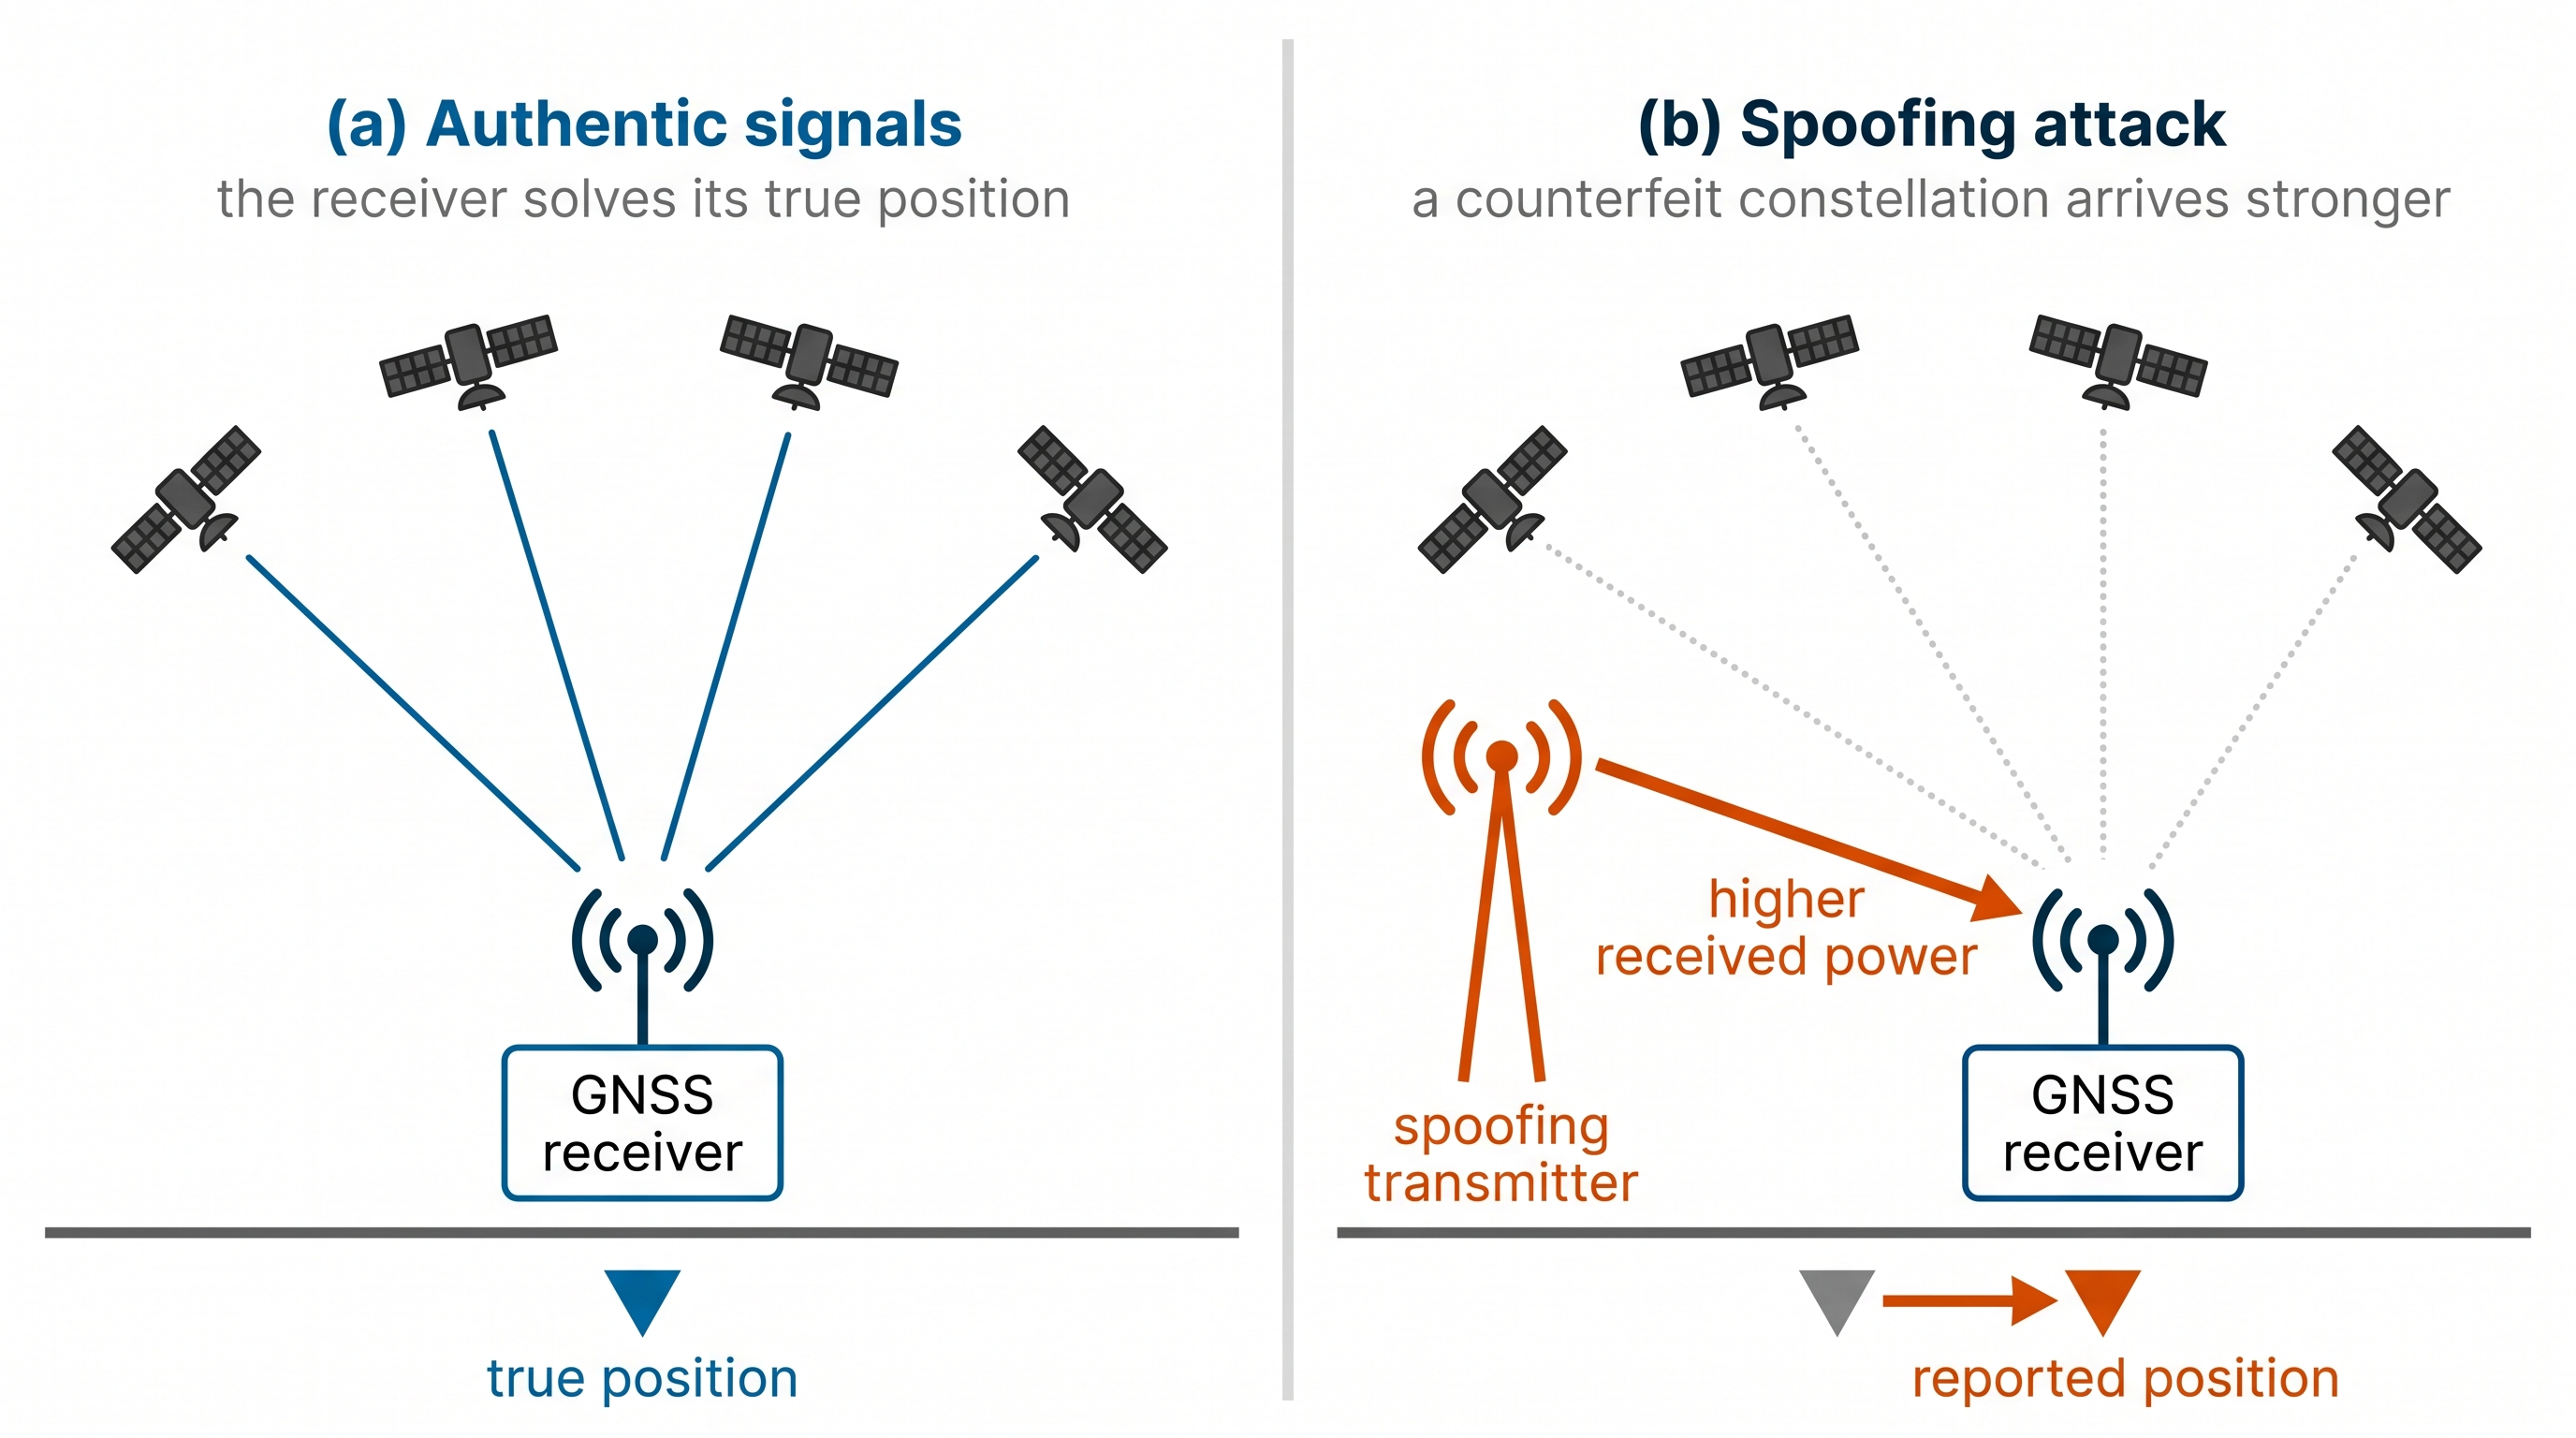
\includegraphics[width=\textwidth]{figures/fig_spoofing_geometry.png}
\caption{A GNSS receiver under authentic signals and under a spoofing attack. In (a) the receiver solves its true position from the satellite signals. In (b) a spoofing transmitter emits a counterfeit constellation that arrives at higher received power, captures the tracking loops, and moves the reported position while the receiver continues to report a valid solution.}
\label{fig:geometry}
\end{figure*}

% Figure source: figures_src/static/fig01_pipeline (hand made, distributed by
% figures_src/sync.py). Do not edit the copy inside figures/, it is overwritten.
\begin{figure*}[t]
\centering
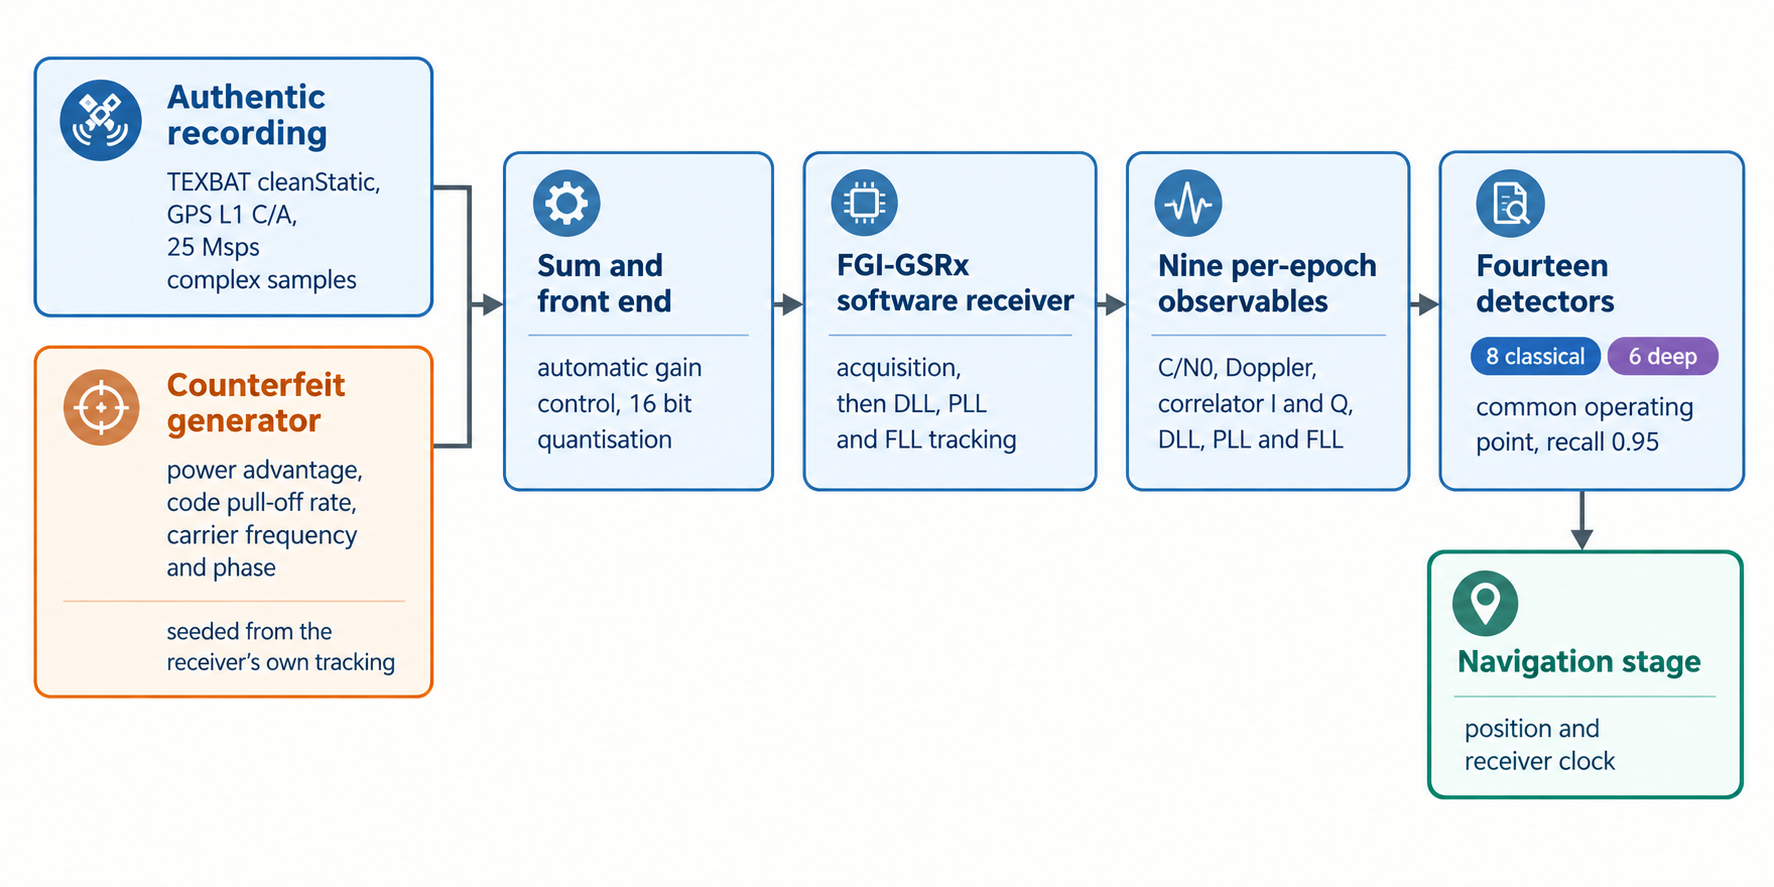
\includegraphics[width=\textwidth]{figures/fig01_pipeline.jpeg}
\caption{How a transmitted attack becomes a detector input. A counterfeit GPS L1 C/A
signal is generated as radio samples and added to authentic recorded samples. The sum
passes through the front end and is tracked by the FGI-GSRx software receiver, which
produces the nine per-epoch measurements the detectors read. The same tracking output
also feeds the navigation stage, which yields the position and the receiver clock.}
\label{fig:pipeline}
\end{figure*}

Evaluating at the waveform level fixes the relationship between the adversary's actions and
the detector's inputs, for the regime this study addresses. The generator is seeded from the
receiver's own tracking of the authentic recording, so the counterfeit arrives aligned, and
the evaluation therefore characterises detector behaviour conditional on an adversary having
achieved that alignment. Achieving it is a separate problem, and the results here should be
read as conditional on capture and not as an end to end demonstration. The adversary acts on transmitter settings, listed in
Table~\ref{tab:attacker}, which are the quantities a physical spoofer controls; the
observables follow from a receiver tracking the resulting signal, and inherit whatever
dependencies receiver processing imposes on them. Several of the observables a detector
reads are computed from the same underlying correlator output and therefore cannot be varied
independently, so the mapping from adversary action to detector input is not the identity
and is not free. The generator is validated against data set ds7 of the battery, a recorded
attack whose construction is documented in full \citep{humphreys2016texbatds78}, and
reproduces the observables recorded for it.

All fourteen detectors are placed at a common operating point, defined as the highest
decision threshold at which a detector still flags 95 percent of spoofed samples on clean
validation data. A common operating point is necessary because a classifier's error rates
move together with its threshold, so detectors read at different thresholds are not
comparable. The false alarm rate each detector pays to meet the recall floor is reported
alongside every result.

Three findings follow. First, ranking on clean data inverts under transmitted attack: the
random forest attains the highest clean $F_1$ score, the harmonic mean of precision and
recall, and the lowest false alarm rate, yet fails to flag 55 of the 126 transmitted attacks
that capture the receiver, flagging as few as 0.1 percent of the spoofed samples of one of
them. Second, the detectors that flag every attack achieve this only by flagging 46 to 74
percent of authentic data, a regime in which a receiver would alarm almost continuously, so
their apparent resistance is not operationally available. Across all fourteen, false alarm
rates at this operating point span 34 to 96 percent. Third, a missed attack propagates to
the navigation solution: followed through the navigation stage, one such attack drives the
receiver clock at 48.89 nanoseconds per second against a commanded 48.87, after the
receiver's own drift of 0.12 nanoseconds per second has been measured and removed.

\subsection{Contributions}

The principal contribution is the evaluation methodology, because the findings that
follow hold only if the detector inputs are produced by receiver processing of a
signal an adversary could transmit. The remaining four rest on it: the second supplies
the adversary's choice set, the third and fourth measure what existing detectors do
against that choice set and what a failure costs, and the fifth relates the result to
the feature space evaluation the literature more commonly reports.

\begin{enumerate}
  \item \textbf{An evaluation methodology in which every attack is a transmitted
  waveform.} Each attack is synthesised as radio samples, summed with authentic
  recordings and tracked by a software receiver, so that the detector inputs are
  produced by receiver processing of a transmittable waveform. The generator is
  validated by reproducing a recorded attack whose construction is published.

  \item \textbf{A library of transmitted attacks.} Two hundred and nine transmitter
  settings spanning counterfeit power, code pull-off rate and carrier alignment, of
  which 126 satisfy the published conditions for receiver takeover. The library
  expresses the adversary's choice set as data and separates transmissions that
  capture a receiver from those that do not.

  \item \textbf{A comparative evaluation of fourteen detectors,} eight classical and
  six deep, against that library at a common operating point, reporting for each
  detector the number of transmitted attacks it fails to flag together with the false
  alarm rate it incurs on authentic data, with exact binomial intervals on every
  count.

  \item \textbf{A navigation domain measurement} establishing that a missed attack
  reaches the position and timing solution, obtained by propagating one such attack
  through the navigation stage and comparing the induced clock drift against the rate
  the transmitter was configured to impose.

  \item \textbf{A comparison against feature space evaluation,} in which the same
  detectors are attacked by perturbing measurements directly. The two views agree on
  which detectors are fragile, and disagree on the support vector machine, whose
  apparent resistance is accounted for by its false alarm rate. A perturbation size
  reported without that rate would invert the conclusion.
\end{enumerate}

\subsection{Organisation}

Section~\ref{sec:related} reviews spoofing detection and the robustness of learned
classifiers. Section~\ref{sec:signal} describes the receiver processing chain and the
observables it produces. Section~\ref{sec:threat} defines the threat model and the attack
space. Section~\ref{sec:method} presents the waveform generator, its validation, the attack
library, the detector set and the operating point calibration.
Section~\ref{sec:results} reports the results, Section~\ref{sec:discussion} examines their
implications for receiver integrity and states the scope of the study, and
Section~\ref{sec:conclusion} concludes.

\section{Related Work}
\label{sec:related}

\subsection{Classical spoofing detection}
\label{sec:rw_classical}

Classical anti-spoofing tests operate on quantities the tracking loops already produce,
which makes them inexpensive to compute and straightforward to interpret. Received power
monitoring compares the carrier-to-noise density ratio $C/N_0$ against the value expected
for a satellite at a given elevation; a counterfeit transmitted above the authentic power
raises this quantity, and the additional energy also registers in the automatic gain
control setting of the front end \citep{akos2012gnss}. Correlation shape tests examine the
peak formed when the incoming signal is correlated against a locally generated replica of
the spreading code. An authentic signal yields a symmetric peak whose width is set by the
chip duration and the front end bandwidth, whereas a counterfeit present alongside the
authentic signal superimposes a second peak and distorts the composite, producing
asymmetry that can be quantified from early, prompt and late correlator taps
\citep{psiaki2016gnss}. Consistency tests exploit relations that must hold among
measurements of a genuine signal: the code and carrier observables of one satellite track
the same changing geometric range and must therefore evolve together, so a counterfeit
that displaces one without the other violates the relation \citep{psiaki2016gnss}.

How much of the adversary's parameter space these tests actually cover has itself been
measured, and the answer is not all of it. The detection rate of signal quality monitoring
metrics falls for particular combinations of counterfeit code phase and carrier phase, and
metrics formed from several correlator offsets have been proposed to widen that coverage,
reaching a reported 96.1 percent across those combinations \citep{wu2025musd}. Reading the
correlator output as an eye diagram is reported to increase coverage by more than 60
percent over signal quality monitoring and carrier-to-noise density tests
\citep{wu2025eyediagram}. What a classical test achieves therefore depends on where in its
parameter space the spoofer chooses to operate. The present paper asks the same question of
learned detectors, and asks it of transmissions that satisfy the conditions for capturing a
receiver.

These tests are complementary in the sense that no one of them subsumes another, and a
receiver running several raises the cost of a successful attack. They nonetheless share a
structural property. Each is defined by a single named physical signature, which is what
makes it interpretable, and a spoofer that maintains the named quantity within its nominal
range satisfies the test. Because the family of deployed tests is documented in the open
literature, an adversary can treat the signature set as known and design a transmission
that respects it. This observation motivates detection rules that are not specified in
advance by a human.

\subsection{Machine learning based spoofing detection}
\label{sec:rw_learning}

A learned detector replaces a hand specified statistic with a decision rule inferred from
labelled data. A receiver is run over recordings in which the ground truth is known, each
epoch yields a feature vector of the observables available at that instant together with a
label, and a classifier is fitted to reproduce those labels before being applied to unseen
epochs. Because the classifier consumes the observables jointly, it can respond to
configurations that no univariate statistic encodes.

Two model families recur in this literature, and both are represented in the present
study. Single epoch classifiers operate on one observation vector at a time. Decision
trees partition the feature space by recursive threshold tests, and ensembles such as
random forests and gradient boosted trees aggregate many such partitions to reduce
variance. Nearest neighbour classifiers assign a label from the closest training examples,
and support vector machines construct a maximum margin separating surface, in the
nonlinear case through a kernel. Sequence models instead consume a window of consecutive
epochs and can therefore exploit temporal structure. Convolutional networks extract local
patterns across the window, recurrent architectures such as the long short term memory
propagate state along it \citep{hochreiter1997long}, and attention based architectures
weight the epochs of the window against one another \citep{vaswani2017attention}.

Applications to GNSS spoofing span both families. Deep networks have been applied to
correlator outputs \citep{borhanidarian2024deep}, to signal quality features on small
uncrewed aircraft \citep{sung2022cnn}, to receiver exchange format records
\citep{romaniuc2025lstm} and to unmanned aerial platforms \citep{yang2025deep}. Classical
models have been applied through support vector machines \citep{chen2022svm}, nearest
neighbour classifiers \citep{mahroof2024ml} and feed forward networks benchmarked against
recurrent alternatives \citep{jullian2022deep}. Real time operation has been addressed
\citep{li2025realtime}, as has enlargement of the training distribution by generative
augmentation \citep{chen2025cgan}. Reported detection accuracy across this body of work is
consistently high, and the architectures achieving it are heterogeneous, which suggests
that the reported figures are substantially determined by the evaluation corpora and
not by architectural choices.

\subsection{Generalization beyond the training attacks}
\label{sec:rw_generalization}

A classifier fitted to recorded examples characterises the attacks contained in those
recordings, and whether its accuracy persists on an attack outside them is a separate
question that has received direct attention.

One response treats detection as one class learning, fitting only the authentic
distribution so that any sufficiently atypical observation is flagged, which removes the
dependence on a catalogue of attack examples \citep{iqbal2024deep}. A second augments the
training set with synthetically generated attacks in order to widen the distribution the
detector has seen \citep{chen2025cgan}. A third constrains the detector with physics.
Code carrier consistency, the same relation the classical consistency test evaluates, has
been imposed as a training constraint, so the network must respect a relation authentic
signals satisfy. This is reported to preserve accuracy across held out scenarios on which
unconstrained detectors degrade \citep{song2026generalized}.
The appeal of the third approach is that a physically grounded invariant does not depend
on which attacks were recorded.

This line of work addresses distribution shift, in which the test attacks are drawn from a
different distribution than the training attacks but are still drawn and not chosen.
Adversarial selection is a distinct axis: the attack is not sampled from any distribution
but optimised against the deployed system. The two questions are complementary, and a
library of transmitted attacks of the kind constructed here provides material against
which invariant based detectors can subsequently be examined.

\subsection{Adversarial robustness of learned classifiers}
\label{sec:rw_adversarial}

Classifiers fitted to data can be driven across their own decision boundaries by small,
deliberately chosen input perturbations, an observation that originated in image
classification and has since been shown to be general
\citep{szegedy2014intriguing,goodfellow2015explaining}. The associated literature covers
attack construction under model access \citep{madry2018towards}, methodological standards
for evaluating defensive claims \citep{carlini2019evaluating}, and the framing of the
problem as a security question \citep{biggio2018wild}.

Two results from this literature bear directly on the evaluation of spoofing detectors.
The first concerns adversary knowledge. Attacks that differentiate the loss require access
to model parameters, whereas decision based attacks require only the classifier's output
label and are nonetheless effective \citep{brendel2018decision,chen2020hopskipjump}. A
model that withstands a gradient attack has therefore not been shown robust, because a
model that supplies uninformative gradients may still be crossed by a search that queries
only decisions, a failure mode termed gradient masking \citep{athalye2018obfuscated}. The
second concerns cost. Apparent robustness obtained by displacing a decision threshold is
not a gain, since any classifier can be made difficult to cross by flagging nearly all
inputs; the accuracy and robustness of a fitted classifier trade against one another
\citep{tsipras2019robustness}. A robustness claim is therefore interpretable only when
reported jointly with the false alarm rate that purchased it, and the present study adopts
that convention throughout.

\subsection{Physical realizability and the evaluation gap}
\label{sec:rw_physical}

Transferring these results to a sensing system introduces a requirement absent from the
image setting. A perturbation expressed as a displacement of a feature vector corresponds
to an attack only if some physical action on the sensor produces that displacement.
Research on other sensing modalities has addressed this by constructing attacks in the
physical domain, including against automotive ranging sensors
\citep{petit2015remote,cao2021invisible}, against speech recognition
\citep{carlini2018audio} and against synthetic aperture radar imagery \citep{lin2023sar}.
In the GNSS setting, adversarial perturbation of detector inputs has been reported
\citep{an2025adversarial}.

For a GNSS receiver the requirement is stringent, because the observables a detector reads
are not independent coordinates. Several are computed from the same correlator
accumulations within a single integration period, so displacing one while holding the
others fixed describes a receiver state that no incident waveform produces. Establishing
that a given feature space perturbation is realizable therefore requires an argument about
receiver processing that is specific to the observable set in use. Evaluating at the
waveform level removes the need for such an argument by construction, since the adversary
acts on transmitter parameters and the observables are whatever the receiver computes while
tracking the resulting signal. This is the approach adopted in the present study, and
Section~\ref{sec:res_compare} reports the corresponding feature space evaluation alongside
it so that the two can be compared directly.

\section{Receiver Observables and Signal Tracking}
\label{sec:signal}

The detectors evaluated here operate on observables a receiver computes while tracking a
signal. This section specifies the processing that produces them, the observable set
retained, the criterion by which that set was selected, and the labelling procedure, so
that the effect of a transmitted attack on each quantity can be traced through the chain.

\subsection{Receiver processing}

A GPS L1 C/A satellite transmits a carrier modulated by a pseudorandom spreading code of
1023 chips repeating every millisecond, and by navigation data at 50 bits per second. The
code is public and distinct for each satellite, which is what permits a counterfeit to be
generated at all.

Reception proceeds in two stages. In acquisition the receiver searches jointly over code
phase and carrier frequency until it finds the alignment at which its locally generated
replica correlates strongly with the incoming signal. In tracking it maintains that
alignment as the satellite geometry and the receiver clock evolve. Tracking is implemented
by three feedback loops operating concurrently. The delay locked loop maintains code
alignment by correlating the incoming signal against early, prompt and late replicas and
steering so that the early and late correlations remain equal, which holds the prompt
replica on the correlation peak. The phase locked loop maintains carrier phase alignment.
The frequency locked loop performs the equivalent function for carrier frequency and is
more tolerant of low signal to noise ratio, so it assists when phase lock is marginal.

The loops produce a set of quantities at each integration interval. These quantities are
the detector inputs used throughout this study. They are not selected for convenience of
classification: they are what the receiver computes in order to function, and a detector
operating inside a receiver would have access to precisely this set.

\subsection{Observable measurements}
\label{sec:features}

Table~\ref{tab:features} lists the nine measurements, exported once per epoch for each
tracked satellite.

\begin{table}[t]
\centering
\caption{The nine measurements each detector reads, per satellite per epoch.}
\label{tab:features}
\begin{tabular}{@{}llp{5.1cm}@{}}
\toprule
Measurement & Units & What it is \\
\midrule
$C/N_0$              & dB-Hz  & Received signal strength relative to the noise density \\
Mean $C/N_0$         & dB-Hz  & The same, averaged over the preceding second \\
Noise estimate       & --     & Correlator output away from the peak, used as the noise
                                reference \\
Doppler              & Hz     & Frequency offset of the carrier from its nominal value \\
Prompt in phase      & --     & Correlation with the on peak code copy, in phase
                                component \\
Prompt quadrature    & --     & The same, quadrature component \\
Delay lock discriminator & chips & Difference between the early and late correlations,
                                the code tracking error \\
Phase lock indicator & --     & How well the phase locked loop is holding \\
Frequency lock indicator & -- & How well the frequency locked loop is holding \\
\bottomrule
\end{tabular}
\end{table}

The set spans the three aspects of tracking that a spoofing attack perturbs. Received
power is represented by the first three entries, which respond to the counterfeit's
transmitted power relative to the authentic signal. Carrier behaviour is represented by
the Doppler, the two prompt correlator components and the phase and frequency lock
indicators, which respond to the counterfeit's carrier frequency and phase. Code behaviour
is represented by the delay lock discriminator, which responds to the displacement between
the counterfeit code and the authentic code and therefore to the pull-off rate.
Figure~\ref{fig:featdist} shows the marginal distribution of each observable under the two
classes; the classes overlap in every single observable, which is why a learned detector
that combines them can outperform any univariate threshold.

% Figure source: figures_src/fig_legacy.py
\begin{figure*}[t]
\centering
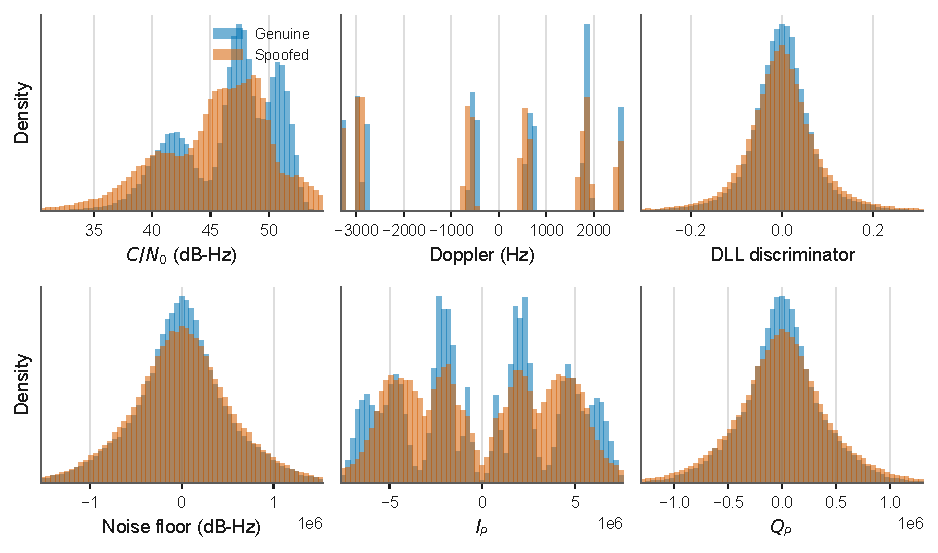
\includegraphics[width=\textwidth]{figures/fig03_feature_distributions.pdf}
\caption{Distribution of each of the nine measurements for authentic and for spoofed epochs. The classes overlap in every measurement, which is why a detector combines them instead of thresholding any one.}
\label{fig:featdist}
\end{figure*}

\subsection{Selection of the observable set}

A software receiver exposes more quantities than the nine retained, and several of the
additional ones are exact deterministic functions of quantities already in the set. The
prompt correlator power is the sum of squares of the two prompt components; the prompt
phase is the arctangent of their ratio; the carrier frequency is the Doppler displaced by
a fixed nominal value.

Such derived quantities are excluded, for two reasons. They contribute no information
beyond their parents, so their inclusion cannot improve an optimal classifier. More
importantly, their presence would admit an evaluation artefact: a perturbation that
displaced a derived quantity without correspondingly displacing its parents specifies a
receiver state that no incident waveform can produce, and any attack exploiting such a
displacement would be an artefact of the feature representation. The nine retained
observables are functionally independent, in the sense that none is an exact function of
the others, which eliminates that particular failure mode.

Functional independence is a property of the representation and does not by itself
establish that an arbitrary configuration of the nine is physically attainable, since
independence among coordinates says nothing about the image of the map from transmitter
parameters to observables. In the waveform level evaluation the question is not reached,
because the observables are by construction whatever the receiver computes while tracking
a transmitted signal. It is reached in the feature space comparison of
Section~\ref{sec:res_compare}, and is treated there.
Figure~\ref{fig:timehistory} shows the joint evolution of the observables for one satellite
across the onset of a recorded attack.

% Figure source: figures_src/fig_legacy.py
\begin{figure*}[t]
\centering
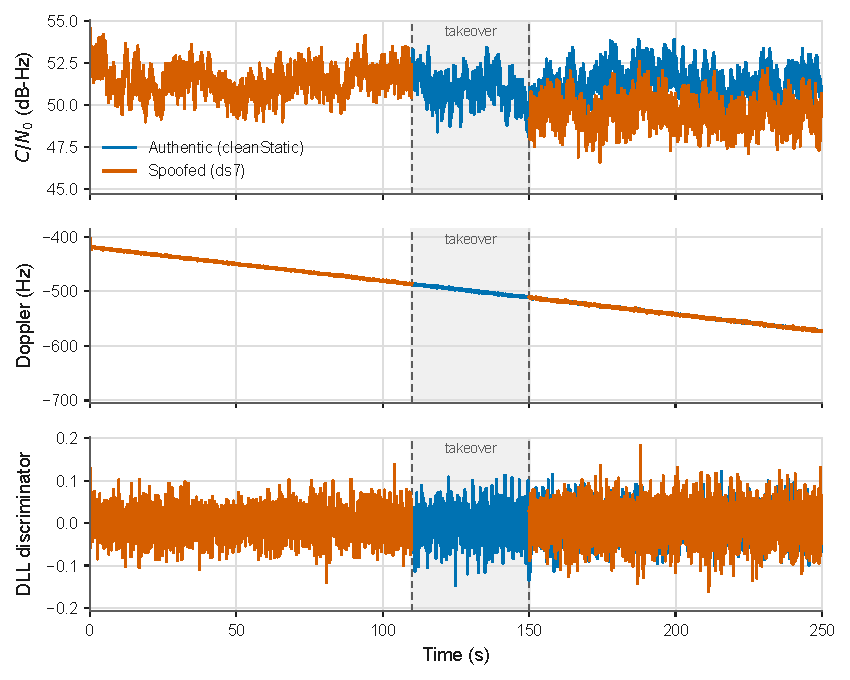
\includegraphics[width=\textwidth]{figures/fig02_signature_timehistory_prn23.pdf}
\caption{Time history of the measurements for one satellite, pseudorandom noise (PRN) code 23, across the onset of a recorded attack. The measurements move together as the counterfeit takes over the tracking loops, which is the signature a detector reads.}
\label{fig:timehistory}
\end{figure*}

\subsection{Labelling and data partitioning}

Each epoch is labelled according to whether the signal being tracked at that instant was
authentic or contained a counterfeit, following the documented onset time within each
recording. Epochs spanning the takeover transient are discarded, because during handover
the tracked signal is neither fully authentic nor fully under the adversary's control and
the label would be ambiguous.

Both classes are drawn from within the same recording. This is a deliberate constraint on
corpus construction. Were authentic epochs taken from one recording and spoofed epochs
from another, a classifier could attain high apparent accuracy by identifying the
recording of origin through front end, antenna or clock characteristics, which is not
spoofing detection and would not transfer to deployment. Drawing both classes from a
single recording, with a common front end and a common clock, removes that confound.

Training, validation and test partitions are taken as disjoint contiguous blocks in time,
with a margin discarded at each boundary. Adjacent epochs of the same satellite are
strongly correlated, since the observables evolve continuously and the integration
interval is short relative to the dynamics, so a randomised partition would place near
duplicates of the same observation on both sides of the split and inflate the measured
accuracy.

\section{Threat Model and Attack Space}
\label{sec:threat}

This section defines the adversary, the parameters under its control, the conditions its
transmission must satisfy to capture a receiver, and the knowledge it is assumed to
possess. Every adversary action in this study is a choice of transmitter settings, so the
threat model is stated in terms of a transmitter and not in terms of a displacement in
a feature space.

\subsection{Adversary model and objective}

The adversary is a spoofer: a transmitter emitting counterfeit GPS L1 C/A signals towards
a victim receiver. Its objective is to cause the victim to report a position or a time of
the adversary's choosing while the victim continues to operate nominally, producing a
converged navigation solution with residuals of ordinary magnitude.

The adversary's only channel to the victim is the radio interface. It does not modify the
victim's software, read its internal state, or alter the observables the victim computes.
Its influence on those observables is mediated entirely by the receiver's own acquisition
and tracking of the composite signal, which is what determines the adversary's variables
in this study.

\subsection{Transmitter controlled parameters}

Table~\ref{tab:attacker} lists the parameters the adversary sets. A choice of all five
defines one attack.

\begin{table}[t]
\centering
\caption{The attacker's controls. Each row is a transmitter setting, not a property of
the victim's measurements. One choice of all five defines one attack.}
\label{tab:attacker}
\begin{tabular}{@{}llp{8.5cm}@{}}
\toprule
Setting & Symbol & What it does \\
\midrule
Power advantage      & $\alpha$   & Strength of the counterfeit relative to the
                                    authentic signal, in decibels \\
Code offset          & $\tau_0$   & Alignment of the counterfeit code at the start,
                                    in chips \\
Code pull-off rate   & $\dot\tau$ & Rate the counterfeit code is dragged away from the
                                    authentic code \\
Carrier offset       & $\Delta f$ & Frequency of the counterfeit carrier relative to
                                    the authentic carrier \\
Carrier phase        & $\phi_0$   & Phase of the counterfeit carrier relative to the
                                    authentic carrier \\
\bottomrule
\end{tabular}
\end{table}

Two of these parameters carry the attack. The power advantage $\alpha$ determines whether
the victim's tracking loops transfer to the counterfeit at all, and the pull-off rate
$\dot\tau$ determines how rapidly the victim's reported range moves once transfer has
occurred. One chip of GPS L1 C/A code corresponds to
$c/f_\mathrm{chip} = 293.05$~m of range, where $c$ is the speed of light and
$f_\mathrm{chip} = 1.023$~MHz is the chipping rate, so a pull-off rate expressed in chips
per second converts directly to metres per second of induced range error. The remaining
three parameters govern the alignment of the counterfeit at onset, and therefore govern
whether the capture conditions of Section~\ref{sec:takeover} are met.

\subsection{Receiver takeover conditions}
\label{sec:takeover}

The adversary cannot select these parameters arbitrarily and still capture a receiver that
is already tracking the authentic signals. Two conditions govern capture
\citep{psiaki2016gnss,kerns2014uav}.

The counterfeit must arrive aligned with the authentic signal in code phase, carrier phase
and Doppler frequency, so that the victim's correlator observes a single undistorted peak
and not two competing peaks. A misaligned counterfeit does not transfer the tracking
loops; it perturbs the victim's observables without displacing its position or time
solution, and therefore constitutes interference and not spoofing. The counterfeit must
additionally exceed the authentic signal in received power, since code tracking follows the
dominant correlation peak. In practice the power advantage employed is small, typically a
few decibels, because a large advantage is itself observable in the receiver's automatic
gain control and in the reported $C/N_0$. This second condition is the established one
and is adopted here, though it may not be necessary: a spoofing method has since been
reported that uses controlled destructive multipath to pull the code loop at a power
below the authentic signal \citep{liu2026dimas}. Requiring the power advantage therefore
makes the attack library used here a conservative subset of what an adversary may
transmit.

Only once both conditions hold does the adversary begin to displace the code. The
experiments in this paper begin from that point: the generator is seeded from the victim's
own tracking so that the alignment condition is satisfied by construction, and what is
measured is detector behaviour after capture has been achieved and not the difficulty
of achieving it. These
conditions define the subset of the parameter space in which an attack is operative, and
Section~\ref{sec:method} applies them to partition the swept library into transmissions
that capture the receiver and transmissions that do not. Detector performance is reported
on the former, so that no detector is credited for flagging a transmission that would not
have succeeded.

\subsection{Knowledge and access assumptions}

The adversary is assumed to have no knowledge of the victim's detector. It does not know
which of the fourteen detectors is deployed, what data that detector was trained on, what
decision threshold it uses, or what score it assigns to any observation. No gradient of any
detector is computed and no detector is queried at any point in the attack construction.

In the taxonomy of Section~\ref{sec:rw_adversarial} this is weaker than a decision based
adversary, which at least observes the classifier's output label. It corresponds to a
spoofer transmitting without feedback from the victim, which is the operationally
realistic case for an attack on a receiver whose alarm state is not externally visible. The
detection failures reported in Section~\ref{sec:results} are therefore failures against an
adversary with no information about the system it defeats.

\subsection{Scope of the adversary model}

Four further restrictions delimit the adversary modelled here relative to the capability a
spoofer may possess in general.

\begin{itemize}
  \item \textbf{No detector knowledge.} As stated above, the transmission is not shaped
  against any specific model.
  \item \textbf{All tracked satellites are spoofed.} An adversary that leaves one
  satellite authentic gains an additional degree of freedom, at the cost of an
  inconsistency between that satellite and the remainder which a cross satellite check may
  identify.
  \item \textbf{A single signal is transmitted}, GPS L1 C/A. A receiver combining multiple
  constellations or multiple frequencies retains evidence that this adversary does not
  attempt to defeat.
  \item \textbf{The victim is stationary and its position is surveyed}, so a common
  pull-off applied to all channels is absorbed into the receiver clock estimate and
  manifests as a timing error.
\end{itemize}

These restrictions determine how the results should be interpreted. Each detection failure
reported in Section~\ref{sec:results} is obtained against this restricted adversary, so the
measured vulnerability is a lower bound on the vulnerability to an adversary that relaxes
any of them. The fourth restriction additionally fixes the observable consequence measured
in Section~\ref{sec:res_nav}: because a common pull-off on all channels is absorbed by the
clock, the induced error appears in the timing solution, and it is that error which is
compared against the commanded rate.

\section{Experimental Methodology}
\label{sec:method}

This section describes how the counterfeit signal is generated, how it is checked
against a recorded attack, how the library of transmitter settings is built, what the
fourteen detectors are, and how they are set to a common operating point.

\subsection{Corpus and receiver configuration}
\label{sec:corpus}

The authentic signal is the cleanStatic recording of the Texas Spoofing Test Battery
\citep{humphreys2012texbat}. It holds raw in-phase and quadrature samples of the GPS L1
band taken at a surveyed stationary antenna, at 25 million complex samples per second
with 16 bits in each component. It contains no spoofing, so it supplies an authentic
signal that a counterfeit can be added to.

All tracking is performed by FGI-GSRx \citep{fgigsrx}, an open software receiver. Using
a published receiver matters for two reasons. The measurements the detectors read are
the ones a real integrity monitor would compute, and any reader can reproduce them from
the same recordings with the same software.

\subsection{Spoofing waveform generation}
\label{sec:generator}

The counterfeit is built as radio samples and then added to the authentic samples.

The generator is seeded from the receiver's own tracking of the authentic recording. For
each satellite the receiver reports, at every millisecond, where it found the code, what
carrier frequency it is tracking and how strong the signal is. Those quantities describe
the authentic signal as the receiver sees it, so they are exactly what a counterfeit
must match in order to arrive aligned. The generator reads them and produces, for each
satellite, a replica of the GPS L1 C/A signal at the same code phase, the same carrier
frequency and the same amplitude.

The attacker's settings of Table~\ref{tab:attacker} are then applied to that replica.
The power advantage scales its amplitude. The code offset and pull-off rate displace its
code, with the displacement growing at the chosen rate. The carrier offset and phase
shift its carrier.

The counterfeit and the authentic samples are summed, and the result passes through a
model of the receiver front end before being written. The front end applies automatic
gain control, which is the mechanism a real receiver uses to keep the signal inside the
range its converter can represent. When added power would drive the sum beyond that
range, the gain is reduced so that the sum still fits. This detail matters. Without it,
added power would clip, and the clipping would be an artefact of the file format instead
of a property of the attack.

The written file is then tracked by FGI-GSRx exactly as the authentic recording is, and
the measurements it produces are what the detectors read.

Two properties follow from building the attack this way. Every constraint a receiver
imposes is satisfied because a receiver produced the measurements, which covers the
continuity of code and carrier, the bandwidth and settling of the tracking loops, the
behaviour of the automatic gain control and the smoothness of the measurements from one
epoch to the next. No projection onto a set of allowed values is applied at any point,
because there is no perturbation to project.
Figure~\ref{fig:rxvalid} shows the checks on the receiver itself.

% Figure source: figures_src/fig_legacy.py
\begin{figure*}[t]
\centering
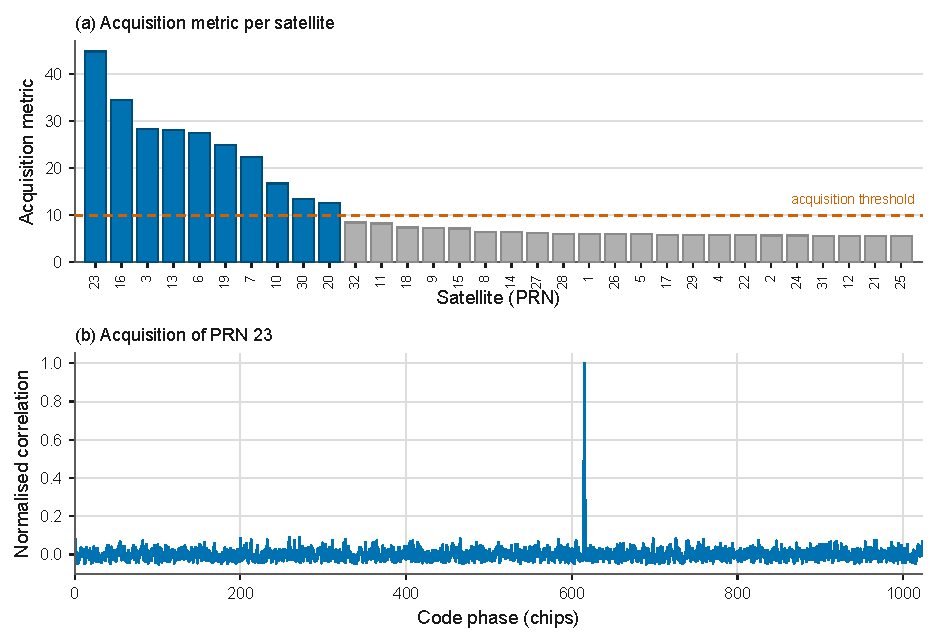
\includegraphics[width=\textwidth]{figures/fig04_receiver_validation.pdf}
\caption{Validation of the software receiver on the authentic recording. Panel (a) shows the acquisition metric for each satellite, and panel (b) shows the correlation against code phase for one satellite. Both match what a correctly operating receiver produces, which establishes that the measurements used throughout come from sound tracking.}
\label{fig:rxvalid}
\end{figure*}

\subsection{Generator validation}
\label{sec:validation}

A generator that cannot reproduce a documented attack is not evidence about attacks that
were never recorded. The check uses data set ds7 of the battery, whose construction is
published in full \citep{humphreys2016texbatds78}.

That document specifies ds7 as a power matched time push carried out with carrier phase
alignment. During the takeover the counterfeit phasor is
$P_s(t) = A_s(t)\,e^{j\theta(t)}$, with the angle $\theta$ rising from $\pi/2$ to $\pi$
and the amplitude following $A_s(t) = -2A_a\cos\theta(t)$, where $A_a$ is the authentic
amplitude. Those two choices together give a combined phasor
\begin{equation}
P_a + P_s = A_a + A_s e^{j\theta} = -A_a e^{j2\theta},
\label{eq:ds7takeover}
\end{equation}
whose magnitude stays at $A_a$ while its angle turns from $0$ to $\pi$. The victim's
loops are therefore walked onto the counterfeit with no step in power and no step in
phase. After the takeover the counterfeit holds at twice the authentic amplitude in
antipodal phase, so the sum returns to magnitude $A_a$, and the document records that
the victim's measurements match the clean recording apart from a carrier phase that is
greater by $\pi$. From then the code is dragged at 1.2 metres per second while the
counterfeit Doppler is held equal to the authentic Doppler.

Running the generator at those settings reproduces the recorded measurements.
Figure~\ref{fig:ds7} reports the comparison. Seven of the eight satellites agree within
half a decibel of carrier-to-noise density ratio. The eighth differs by more, and the
difference is not isolated: across the satellites the gap between generated and recorded
grows with the strength of the satellite, with a Spearman rank correlation of $+0.905$
at $p = 0.002$, and the trend remains when the strongest satellite is removed. The cause
is that the generated counterfeit is an amplitude matched replica, so the cancellation in
Equation~\ref{eq:ds7takeover} is cleaner than the recorded spoofer's hardware achieved,
which leaves the generated attack slightly louder. A slightly louder attack is easier to
detect, so this difference understates what an attacker can do.

\begin{figure*}[t]
\centering
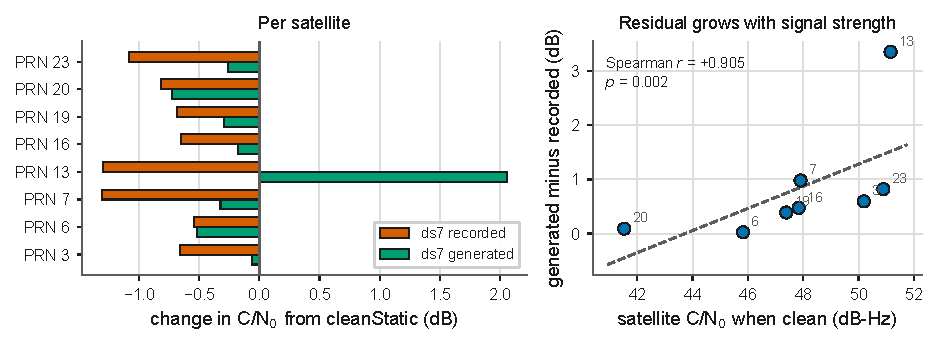
\includegraphics[width=\textwidth]{figures/fig_ds7_validation.pdf}
\caption{The generator reproduces the recorded ds7 attack. Left, the change in
carrier-to-noise density ratio from the clean recording, for the recorded attack and for
the generated one, per satellite. Right, the residual between them grows with satellite
strength, so the strongest satellite is the extreme of a trend and not an isolated
disagreement. The generated attack sits slightly above the recorded one, which makes it
easier to detect.}
\label{fig:ds7}
\end{figure*}

\subsection{Transmitted attack library}
\label{sec:library}

The attacker's choice set is expressed as a library. Each entry is one combination of
the settings in Table~\ref{tab:attacker}, and for each the generator produces a
composite file which the receiver tracks and the exporter turns into measurements. The
library holds 209 entries.

Two families of setting are covered. In the first the counterfeit carrier is in phase
with the authentic carrier, and the power advantage is swept from $-3$ to $10$ decibels.
The second follows the law of Equation~\ref{eq:ds7takeover}: for a counterfeit of
amplitude ratio $g$ at phase $\varphi$, the received power is unchanged when
\begin{equation}
g = -2\cos\varphi ,
\label{eq:neutral}
\end{equation}
so a counterfeit on this locus is invisible to a test that watches received power alone.
The ds7 attack sits on it at $\varphi = \pi$ and $g = 2$. Both families are crossed with
seven code pull-off rates from zero to 147 metres per second and three carrier alignment
settings.

Section~\ref{sec:threat} gives the two conditions a counterfeit must satisfy to take over
a receiver. Applied to the library, they select the entries where the counterfeit is
stronger than the authentic signal and is dragging the code. That is 126 of the 209
entries, and those 126 are the attacks the detectors are measured against.
Figure~\ref{fig:attackspace} shows the library and the subset.

\begin{figure}[t]
\centering
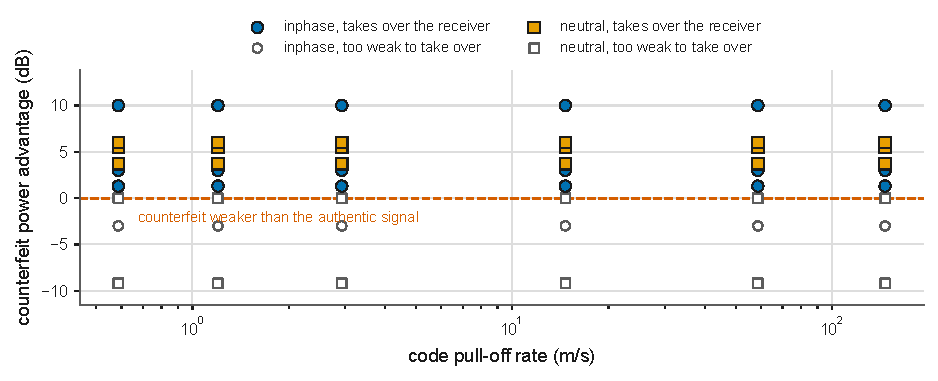
\includegraphics[width=\linewidth]{figures/fig_attack_space.pdf}
\caption{The transmitter settings in the library. Filled markers are the 126 settings
where the counterfeit is stronger than the authentic signal and is dragging the code,
which are the conditions for taking over a receiver. Open markers are settings that do
not meet them. Circles are the in phase family and squares follow the power neutral law
of Equation~\ref{eq:neutral}.}
\label{fig:attackspace}
\end{figure}

\subsection{Detector models and training}
\label{sec:detectors}

Fourteen detectors are tested. They are listed in Table~\ref{tab:detectors} with what
each one does, so that the comparison can be read without reference to the machine
learning literature. All fourteen read the same nine measurements described in
Section~\ref{sec:signal}.

\begin{table*}[t]
\centering
\caption{The fourteen detectors and the decision rule each one applies. The classical
models decide from the measurements of a single epoch. The deep networks decide from a
window of consecutive epochs, so they can use how the measurements change.}
\label{tab:detectors}
\begin{tabular}{@{}p{3.6cm}lp{7.0cm}@{}}
\toprule
Detector & Family & How it decides \\
\midrule
Decision tree      & classical & A sequence of threshold tests on single measurements,
                                 forming one branching rule \citep{breiman2001random} \\
Random forest      & classical & Many decision trees fitted to different samples of the
                                 data, whose votes are averaged \citep{breiman2001random} \\
Gradient boosting  & classical & Trees added one at a time, each fitted to the errors
                                 left by the previous ones \citep{friedman2001greedy} \\
XGBoost            & classical & Gradient boosting with additional penalties on tree
                                 complexity \citep{chen2016xgboost} \\
LightGBM           & classical & Gradient boosting that grows trees leaf by leaf for
                                 speed on large data \citep{ke2017lightgbm} \\
Nearest neighbour  & classical & Labels an epoch by the labels of the most similar
                                 training epochs \\
Support vector machine & classical & Places a boundary separating the classes with the
                                 widest margin, using a radial basis kernel \\
Multilayer perceptron & classical & A small feed forward network of fully connected
                                 layers \\
\midrule
One dimensional convolutional network & deep & Filters slid along the window respond to
                                 local patterns in time \\
Long short term memory & deep & Carries a state along the window, so earlier epochs
                                 inform later ones \citep{hochreiter1997long} \\
Bidirectional long short term memory & deep & The same, traversing the window in both
                                 directions \\
Convolutional recurrent hybrid & deep & Convolutional filters feeding a recurrent
                                 layer \\
Transformer        & deep & Weighs every epoch in the window against every other through
                                 attention \citep{vaswani2017attention} \\
Temporal convolutional network & deep & Dilated convolutions reaching across the window
                                 without recurrence \citep{bai2018empirical} \\
\bottomrule
\end{tabular}
\end{table*}

The set spans the families used in the detection literature reviewed in
Section~\ref{sec:rw_learning}, covering tree ensembles, instance based classification,
kernel methods, a feed forward network and the convolutional, recurrent, hybrid and
attention branches of sequence modelling.

\subsection{Feature space comparison}
\label{sec:comparison}

The attacks described above are transmitted. To show what a study that perturbed the
measurements instead would have concluded, each detector is also measured a second way,
and that measurement is reported alongside as a comparison.

The comparison uses a decision based boundary attack. It is given only the detector's
output decision for a sample, authentic or spoofed, and no gradient, no score and no
knowledge of the model. Starting from a spoofed sample the detector flags, and from an
authentic sample it does not, the attack performs a binary search along the line between
them to locate the point where the decision changes, then reduces the largest single
change across the nine measurements while keeping the decision on the authentic side.
The quantity reported is the smallest such change, measured in the normalised space where
each measurement is scaled to the unit interval, so the nine are comparable.

This is the appropriate comparison to make. A gradient attack would need access to the
detector's internals, and Section~\ref{sec:threat} states that the attacker in this study
has none. A decision based attack needs only the output decision, so it is the strongest
attack available to an adversary that cannot see inside the model
\citep{brendel2018decision,chen2020hopskipjump}. It is also the attack that a
non-differentiable detector cannot evade by denying gradients
\citep{athalye2018obfuscated}.

The comparison is reported for one purpose. It shows where a measurement space
evaluation and a transmitted attack agree about a detector and where they do not, which
Section~\ref{sec:res_compare} sets out. It is not used to support any claim about what a
spoofer can achieve, because a perturbation of the measurements is not by itself a signal
a transmitter can send.

\subsection{Operating point calibration}
\label{sec:oppoint}

A detector reports a score, and a threshold turns that score into a decision. Moving the
threshold trades two quantities against each other. Recall is the fraction of spoofed
samples that are flagged. The false alarm rate is the fraction of authentic samples that
are flagged. Raising the threshold lowers both, and lowering it raises both, so two
detectors read at different thresholds cannot be compared.

Every detector in this study is therefore set to one common operating point. The
threshold is the highest value at which the detector still flags 95 percent of the
spoofed samples in clean validation data,
\begin{equation}
\eta^\star = \max\{\eta : R_\mathrm{val}(\eta) \ge 0.95\},
\label{eq:oppoint}
\end{equation}
where $R_\mathrm{val}$ is recall on that data. A recall floor is the safety first choice
for an integrity monitor, because missing an attack is the failure that matters. The
false alarm rate each detector pays to meet that floor is reported alongside every
result, since a detector can always meet a recall floor by flagging everything.

The data are divided so that training, validation and test come from separate blocks of
each recording, with a gap discarded at every block boundary. Adjacent epochs of the same
satellite are nearly identical, because the tracking loops have time constants of order a
second, so a division that scattered neighbouring epochs across the blocks would place
near copies of the same measurement in training and in test and would inflate every
score.

\section{Results}
\label{sec:results}

Results are reported in four parts. The first is how the detectors perform on clean
data, which fixes the baseline. The second is how they perform against the transmitted
attacks. The third follows one missed attack into the navigation solution. The fourth
compares these measurements against what a perturbation of the measurements alone would
have suggested.

\subsection{Clean performance and false alarm cost}
\label{sec:res_clean}

Every detector is set to the common operating point of Equation~\ref{eq:oppoint}, which
is the highest threshold at which it still flags 95 percent of the spoofed samples in
clean validation data. Table~\ref{tab:main} reports what each detector achieves there.

Two quantities describe clean performance. The $F_1$ score is the harmonic mean of
precision and recall, so it summarises detection quality in one number. The false alarm
rate is the fraction of authentic samples the detector flags, and it is the cost of
meeting the recall floor.

\begin{table*}[t]
\centering
\caption{Every detector at the common operating point of Equation~\ref{eq:oppoint},
ordered by false alarm rate. Passed counts the transmitted take over attacks, out of
126, for which the detector flags fewer than half the spoofed samples. Lowest detection
is the smallest fraction of an attack's samples the detector flagged. The final column
is the smallest perturbation of the measurements alone that crosses the decision
boundary, for comparison.}
\label{tab:main}
\footnotesize
\begin{tabular}{@{}llrrrrr@{}}
\toprule
 & & \multicolumn{2}{c}{Clean data} & \multicolumn{2}{c}{Transmitted attacks}
 & Perturbation \\
\cmidrule(lr){3-4}\cmidrule(lr){5-6}\cmidrule(lr){7-7}
Detector & Family & $F_1$ & False alarm & Passed & Lowest det.
 & $L_\infty$ \\
\midrule
Random forest & classical & 0.833 & 0.337 & 55 (43.7\%) & 0.001 & 0.025 \\
Gradient boosting & classical & 0.827 & 0.350 & 27 (21.4\%) & 0.166 & 0.019 \\
Temporal convolutional & deep & 0.805 & 0.427 & 4 (3.2\%) & 0.469 & 0.041 \\
XGBoost & classical & 0.811 & 0.451 & 28 (22.2\%) & 0.088 & 0.020 \\
Nearest neighbour & classical & 0.800 & 0.462 & 0 (0.0\%) & 0.692 & 0.055 \\
LightGBM & classical & 0.804 & 0.464 & 27 (21.4\%) & 0.151 & 0.021 \\
Decision tree & classical & 0.787 & 0.522 & 21 (16.7\%) & 0.139 & 0.023 \\
Multilayer perceptron & classical & 0.758 & 0.587 & 14 (11.1\%) & 0.171 & 0.039 \\
Bidirectional LSTM & deep & 0.741 & 0.662 & 0 (0.0\%) & 0.712 & 0.064 \\
Long short term memory & deep & 0.735 & 0.679 & 0 (0.0\%) & 0.568 & 0.065 \\
Convolutional recurrent & deep & 0.734 & 0.693 & 0 (0.0\%) & 0.725 & 0.067 \\
Convolutional network & deep & 0.725 & 0.737 & 0 (0.0\%) & 0.636 & 0.058 \\
Transformer & deep & 0.707 & 0.794 & 18 (14.3\%) & 0.004 & 0.058 \\
Support vector machine & classical & 0.682 & 0.960 & 53 (42.1\%) & 0.074 & 0.111 \\
\bottomrule
\end{tabular}
\end{table*}

The random forest achieves the highest $F_1$ score at 0.833 and the lowest false alarm
rate at 0.337. Gradient boosting follows at 0.827 and 0.350. The support vector machine
is last on both counts, at 0.682 and 0.960.

The false alarm rates deserve attention on their own. Across the fourteen detectors they
run from 0.337 to 0.960. Even the best of them flags about a third of authentic samples
as spoofed. On this evidence no detector in the study is usable as a standalone
single epoch integrity monitor, before any attacker is considered. A fielded monitor
would combine decisions over several epochs, trading detection latency for a lower rate
of false alarms, and the per epoch numbers reported here are the input to such a scheme.
Figure~\ref{fig:oppoint} shows the clean scores at that operating point.

% Figure source: figures_src/fig_legacy.py
\begin{figure}[t]
\centering
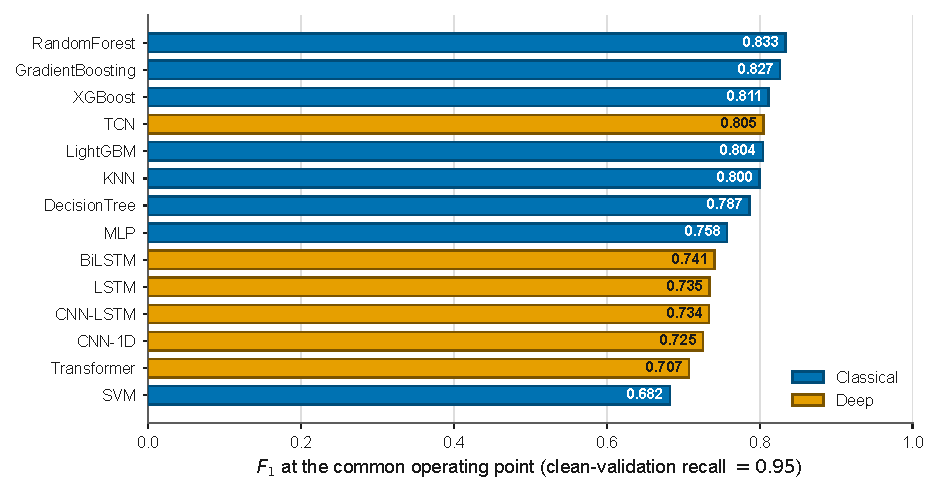
\includegraphics[width=\linewidth]{figures/fig05_detection_operating_point.pdf}
\caption{Clean $F_1$ for every detector at the common operating point, the threshold at which each flags 95 percent of spoofed samples in clean validation data. Classical and deep detectors are interleaved, so no family dominates before an attacker is considered.}
\label{fig:oppoint}
\end{figure}

\subsection{Detector performance under transmitted attacks}
\label{sec:res_attack}

Each detector is then run against the 126 transmitted settings that meet the conditions
for taking over a receiver. For each setting the detection rate is the fraction of that
attack's spoofed samples the detector flags. Because every sample in these files is
spoofed, the detection rate is the detector's recall against that particular attack. A
setting counts as passed when the detector flags fewer than half of its samples.

Table~\ref{tab:main} and Figure~\ref{fig:detection} report the outcome.

\begin{figure}[t]
\centering
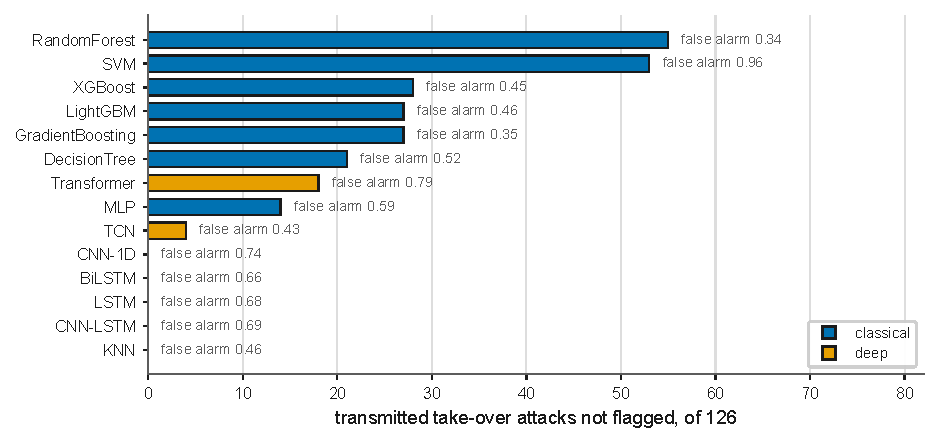
\includegraphics[width=\linewidth]{figures/fig_detection_vs_transmitted.pdf}
\caption{Transmitted take over attacks each detector fails to flag, out of 126. The
clean false alarm rate each detector pays at the common operating point is printed
beside its bar. The detector with the lowest false alarm rate fails to flag the most
attacks.}
\label{fig:detection}
\end{figure}

The detector that performs best on clean data is the one most often passed. The random
forest fails to flag 55 of the 126 attacks, which is 43.7 percent of them. Against one
setting it flags 0.1 percent of the spoofed samples, so the attack is present throughout
and the detector reports authentic almost everywhere.

Gradient boosting fails to flag 27, XGBoost 28 and LightGBM 27. The support vector
machine fails to flag 53, and it does so while flagging 96 percent of authentic samples,
so it is neither accurate nor resistant.

Five detectors flag every one of the 126 attacks. They are the nearest neighbour
classifier, the one dimensional convolutional network, the convolutional recurrent
hybrid, the bidirectional long short term memory and the long short term memory. Their
lowest detection rate against any attack stays between 0.568 and 0.725. Their false alarm
rates on authentic data run from 0.462 to 0.737, so between 46 and 74 percent of
authentic samples are flagged as attacks. Their resistance is bought by flagging a large
part of the authentic data, which is the trade described in
Section~\ref{sec:rw_adversarial} and not a property that could be used in a receiver.

Taken together, no detector in the study is both usable and resistant. The two with the
lowest false alarm rates are passed by 43.7 and 21.4 percent of the attacks. The five
that are never passed carry false alarm rates that rule them out.
Figure~\ref{fig:integrity} places the detectors on the two axes an integrity monitor trades.

% Figure source: figures_src/fig_legacy.py
\begin{figure}[t]
\centering
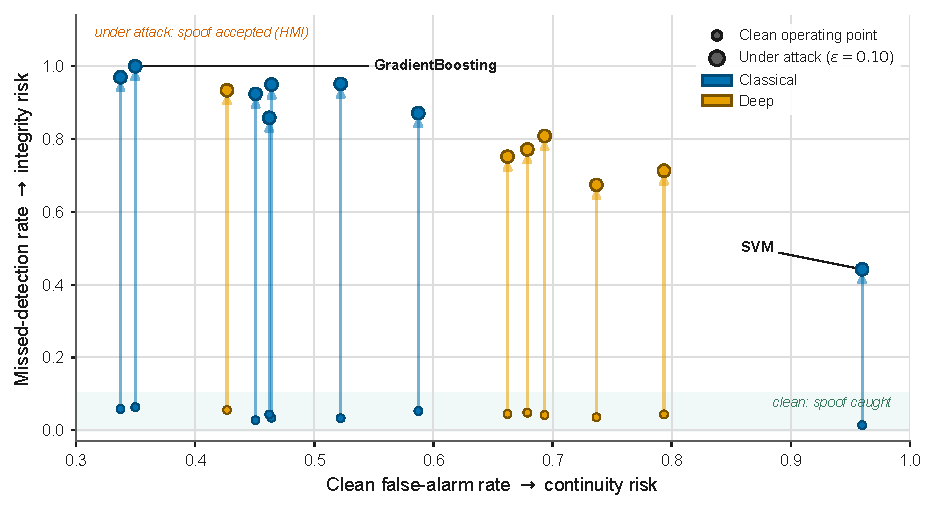
\includegraphics[width=\linewidth]{figures/fig12_integrity_plane.pdf}
\caption{Each detector placed by the two risks a navigation integrity monitor trades. The horizontal axis is the false alarm rate on authentic data, which drives continuity risk. The vertical axis is the missed detection rate, which drives integrity risk. No detector reaches the lower left corner.}
\label{fig:integrity}
\end{figure}

\subsection{A single transmitter setting evading six detectors}
\label{sec:res_single}

The counts above describe an attacker that transmits every setting in turn. A real
attacker chooses one setting and transmits it. The relevant question is therefore what a
single choice achieves.

The best single setting is a counterfeit three decibels stronger than the authentic
signal, in phase with it, dragging the code at 14.65 metres per second. Transmitted once,
it is passed by six of the fourteen detectors at the same time. Those six are the
decision tree, the random forest, gradient boosting, XGBoost, LightGBM and the
Transformer, so every tree based detector in the study is among them, including the one
with the best clean performance, which flags 1.2 percent of the samples.

This is the same setting that Section~\ref{sec:res_nav} follows through the navigation
stage. One transmitted configuration therefore passes six detectors and drives the
receiver clock at the commanded rate. The attacker needs no knowledge of which detector
is running, because this single choice covers six of them.

A second setting, identical except that the code is dragged at 2.93 metres per second,
passes the same six detectors. The attacker can therefore trade the speed of the induced
error against nothing at all, since both rates pass the same set.

\subsection{Navigation domain consequence}
\label{sec:res_nav}

Detection failure matters only if the attack it misses does something. One of the missed
settings is therefore followed through the navigation stage, which is the part of the
receiver that turns the measurements into a position and a clock estimate.

The setting is a counterfeit three decibels stronger than the authentic signal, dragging
the code at 14.65 metres per second. The random forest flags 1.2 percent of its samples.
The attack drags every satellite by the same amount, and a stationary receiver absorbs a
common change in range into its clock estimate, so the expected effect is a drift of the
receiver clock at
\begin{equation}
\frac{\dot\tau \, c/f_\mathrm{chip}}{c} = \frac{14.65}{c} = 48.87~\mathrm{ns/s}.
\label{eq:clockrate}
\end{equation}

The receiver's own clock drift is measured first, by running the same window with the
counterfeit switched off. It is 0.12 nanoseconds per second, so it is negligible against
the rates under test, and it is subtracted from every figure below.

The corrected drift is 48.89 nanoseconds per second against a commanded 48.87, a
difference of 0.02 nanoseconds per second, or 0.05 percent. Figure~\ref{fig:clock} shows the clock
estimate over the window together with the commanded rate. The navigation solution
converged at every epoch with a figure of merit below one metre, so the receiver was
producing an ordinary fix while its clock was being driven.

\begin{figure*}[t]
\centering
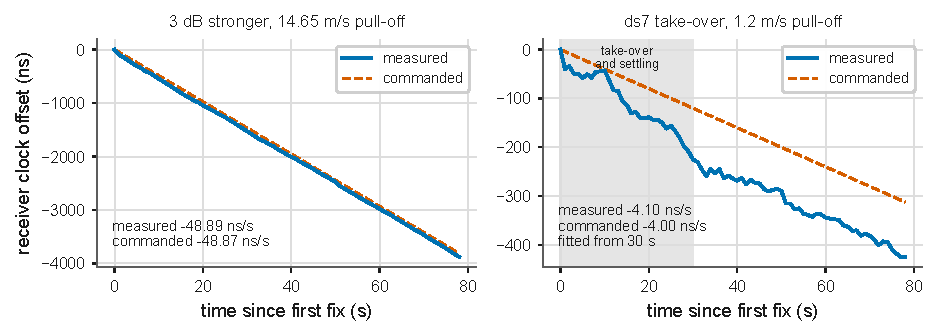
\includegraphics[width=\textwidth]{figures/fig_clock_push.pdf}
\caption{The attack reaches the navigation solution. Receiver clock offset over the
window for two transmitted attacks, with the rate each transmitter was set to impose. In
the left panel the measured drift is within 0.05 percent of the commanded rate. The
detector with the best clean performance reports 98.8 percent of the samples in that
attack as authentic.}
\label{fig:clock}
\end{figure*}

The right panel of Figure~\ref{fig:clock} shows the ds7 takeover at 1.2 metres per
second. This attack carries a takeover of 20 seconds before its code begins to drift, and
the tracking loops need time to settle once they have been captured. Fitting across the
whole window therefore mixes the settling transient with the drift. The measured slope
over successive 20 second segments is $-6.27$, $-7.50$, $-4.72$ and $-4.68$ nanoseconds
per second, so the loops have settled about 30 seconds in.

Fitted after settling, the corrected drift is 4.10 nanoseconds per second against a
commanded 4.00, a difference of 2.3 percent. Both attacks therefore drive the receiver
clock at the rate the transmitter was set to impose, one of them through a takeover and
one without.
Figure~\ref{fig:ladder} sets out what each kind of attack is assumed to know.

% Figure source: figures_src/static/fig_threat_ladder.png (hand made)
\begin{figure*}[t]
\centering
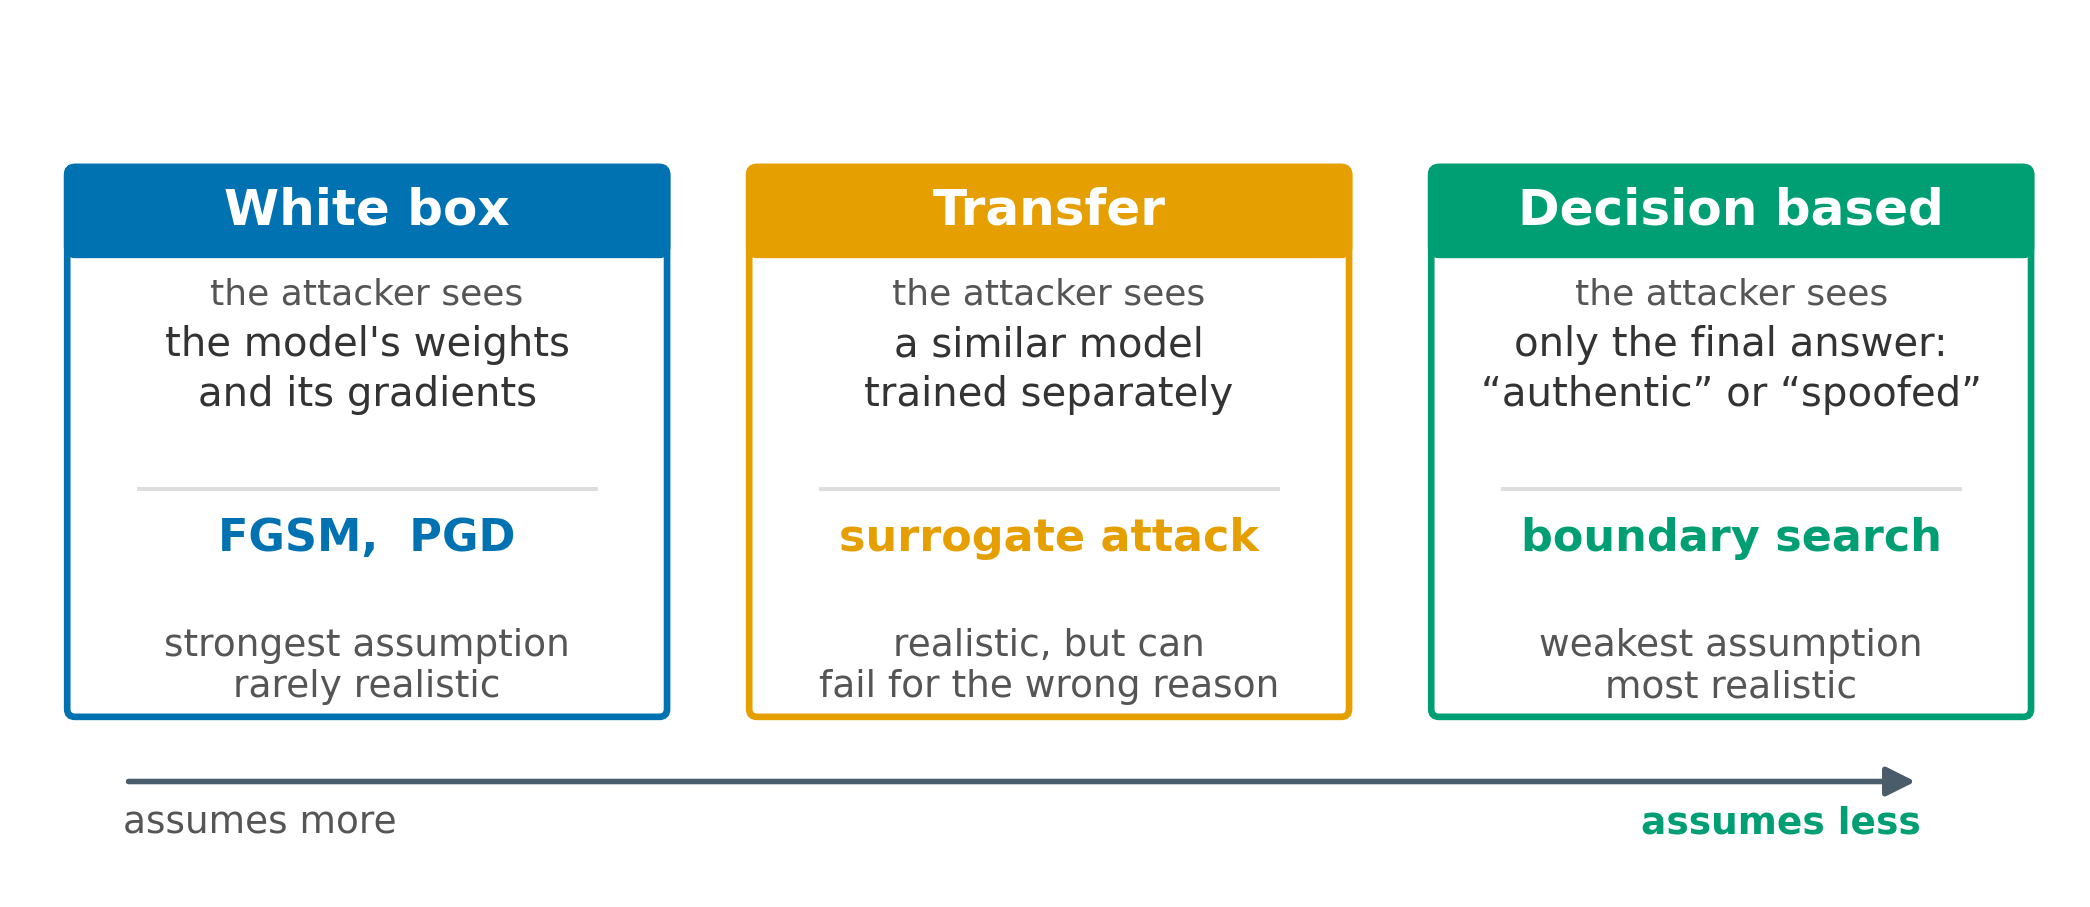
\includegraphics[width=\textwidth]{figures/fig_threat_ladder.png}
\caption{What an attacker is assumed to know. A white box attacker holds the model and its gradients, a transfer attacker holds a separately trained substitute, and a decision based attacker sees only the output decision. The comparison in this section uses the last of these, which assumes least.}
\label{fig:ladder}
\end{figure*}

\subsection{Comparison with feature space evaluation}
\label{sec:res_compare}

The same fourteen detectors were also measured with the decision based boundary attack of
Section~\ref{sec:comparison}, which perturbs the measurements directly without generating
a signal. Table~\ref{tab:main} reports the size of the smallest perturbation that crosses
each detector's decision boundary, expressed in the normalised measurement space.

The two views agree on which detectors are fragile. The tree based detectors need the
smallest perturbations, from 0.019 to 0.025, and they are also the detectors most often
passed by a transmitted attack. The agreement is useful, because it shows the fragility
is a property of those detectors and not an artefact of either measurement.

The two views disagree on the support vector machine. It needs by far the largest
perturbation at 0.111, which taken alone would read as the most robust detector in the
study. Its false alarm rate of 0.960 explains this. A detector that flags almost
everything is hard to push into flagging, and the transmitted measurement shows the same
detector being passed by 53 of the 126 attacks. Reading the perturbation size without the
false alarm rate would have inverted the conclusion.
Figure~\ref{fig:fragility} gives the resulting ranking.

% Figure source: figures_src/fig_legacy.py
\begin{figure}[t]
\centering
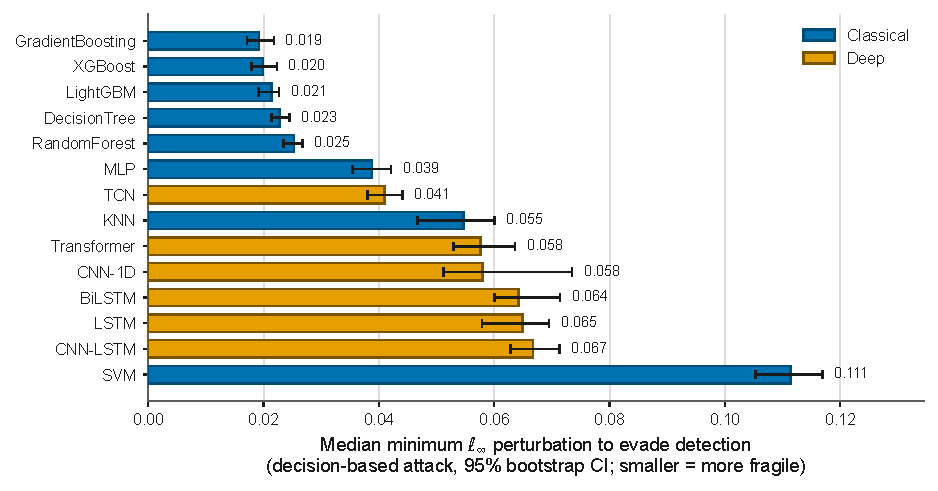
\includegraphics[width=\linewidth]{figures/fig06_fragility_ranking.pdf}
\caption{Median smallest perturbation of the measurements alone that moves each detector across its decision boundary, under the decision based attack. Larger is more resistant. This is the comparison measurement, not the transmitted attack.}
\label{fig:fragility}
\end{figure}
Figure~\ref{fig:rankinv} compares that ranking against the clean one.

% Figure source: figures_src/fig_legacy.py
\begin{figure}[t]
\centering
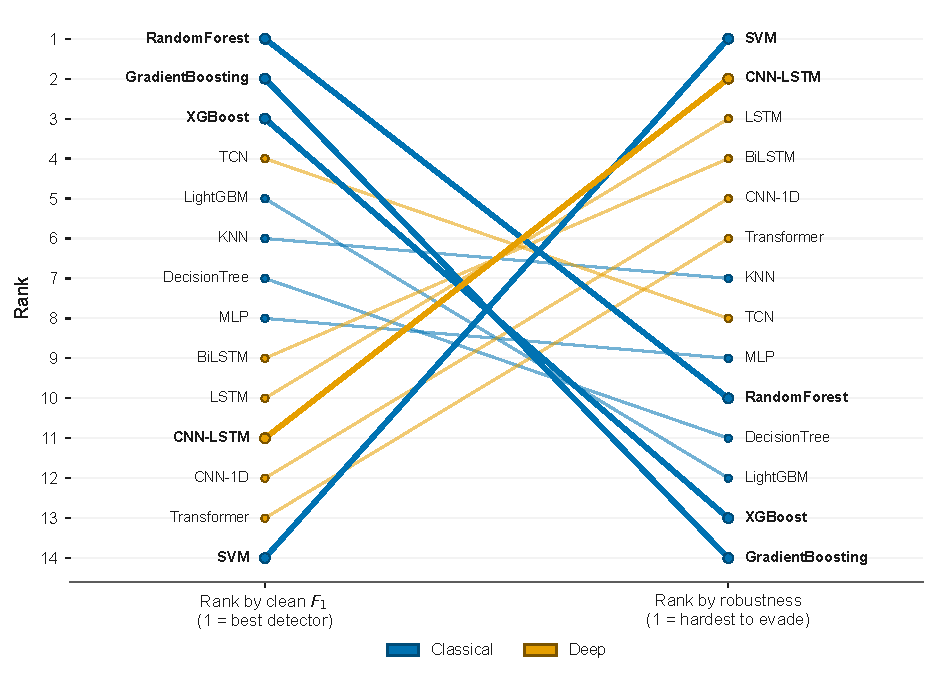
\includegraphics[width=\linewidth]{figures/fig10_rank_inversion.pdf}
\caption{Detectors ranked by clean $F_1$ against the same detectors ranked by resistance to the decision based attack. The two orderings run close to opposite, which is the same relation the transmitted attacks produce.}
\label{fig:rankinv}
\end{figure}

\section{Discussion}
\label{sec:discussion}

\subsection{Principal findings}

Three findings follow from Section~\ref{sec:results}, each obtained against attacks that
were synthesised as waveforms and tracked through the receiver.

Clean detection performance does not predict resistance to transmitted attack. The random
forest attains both the highest clean $F_1$ score and the lowest false alarm rate of the
fourteen detectors, and it is nonetheless evaded by 43.7 percent of the transmitted
takeover attacks, with an exact interval of [0.348, 0.528]. The effect is not confined to
one model: the four detectors with the highest clean $F_1$ are evaded on 0.226 of their
detector-attack pairs against 0.106 for the remaining ten, a difference significant at
$p = 2.8 \times 10^{-10}$. Because all fourteen detectors are read at the same recall
floor, this cannot be attributed to differences in threshold placement, and because the
attacks were selected without reference to any detector, it cannot be attributed to
adversarial optimisation against a particular model.

The relationship is a contrast between groups and not a monotone trend across
architectures. Section~\ref{sec:res_stats} reports a Spearman correlation of $+0.41$
between clean $F_1$ and evaded fraction which is not significant at $n = 14$, because the
support vector machine combines the worst clean score with the second highest evasion
count. Both results are reported, and the contrast is the one the
evidence supports.

Where resistance does appear, it is purchased with false alarms. Five detectors flag every
one of the 126 attacks, and those same five flag between 46 and 74 percent of authentic
samples. A receiver alarming on half of its authentic observations would be
disabled in service, so this resistance is not operationally available, and the pattern is
the accuracy against robustness trade of Section~\ref{sec:rw_adversarial} appearing in a
GNSS setting. Figure~\ref{fig:tradeoff} shows the same point across the full set of
criteria a deployment decision weighs: no detector dominates on all of them, and the
orderings induced by different criteria disagree, so no single scalar ranks the set.

% Figure source: figures_src/fig_legacy.py
\begin{figure}[t]
\centering
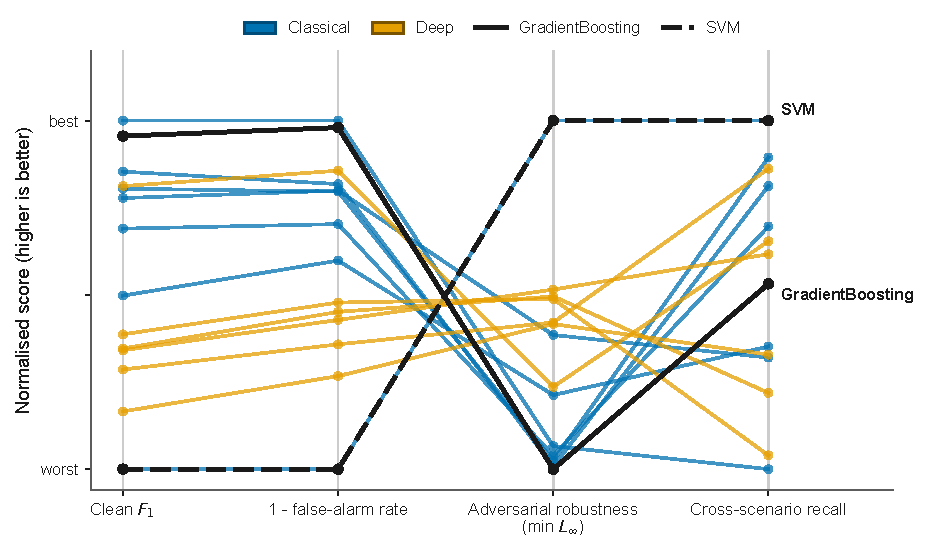
\includegraphics[width=\linewidth]{figures/fig11_tradeoff_parallel.pdf}
\caption{Every detector across the criteria a deployment decision would weigh, each normalised so higher is better. No detector is best on all of them, and the orderings disagree, so a single accuracy figure cannot rank them.}
\label{fig:tradeoff}
\end{figure}

A missed detection is consequential and not benign. The attack propagated through the
navigation stage drove the receiver clock at the rate the transmitter was configured to
impose, to within 0.05 percent, while the detector with the best clean performance
classified 98.8 percent of its samples as authentic. Detection failure and navigation
domain effect were measured on the same attack and the same recording, so the two are not
independent observations juxtaposed after the fact.

\subsection{Implications for detector evaluation}

Evaluating at the waveform level fixes the interpretation of the resulting failure rates.
A displacement applied directly to a table of receiver observables corresponds to an attack
only if some incident waveform produces that displacement. Several observables a receiver
reports are computed from the same correlator accumulations and cannot be varied
independently, so an evaluation that varies them independently may report vulnerability to
a receiver state that no transmission realises. When the attack is generated as a signal,
the observables are by construction whatever the receiver computed while tracking it, and
every constraint receiver processing imposes is satisfied because that processing imposed
it.

Section~\ref{sec:res_compare} quantifies what this changes. For the tree based detectors
the feature space and waveform level evaluations agree, and the fragility those models
exhibit is a property of the models and not of either evaluation. For the support
vector machine the two disagree entirely: its minimum perturbation is the largest in the
study, which taken alone would identify it as the most robust detector, yet it is evaded by
53 of the 126 transmitted attacks. Its false alarm rate of 0.960 reconciles the two
readings, since a classifier that flags almost everything is expensive to cross in feature
space while remaining useless as a monitor. The conclusion is not that one evaluation is
invalid, but that a perturbation magnitude reported without the false alarm rate that
accompanies it can invert the ordering it appears to establish.

A related limitation of accuracy based evaluation appears under distribution shift.
Figure~\ref{fig:generalization} reports recall on data withheld from training, holding out
either an entire attack scenario or individual satellites. Recall falls in both cases,
which indicates that the detectors depend on conditions present in their training data even
before an adversary is introduced.

% Figure source: figures_src/fig_legacy.py
\begin{figure*}[t]
\centering
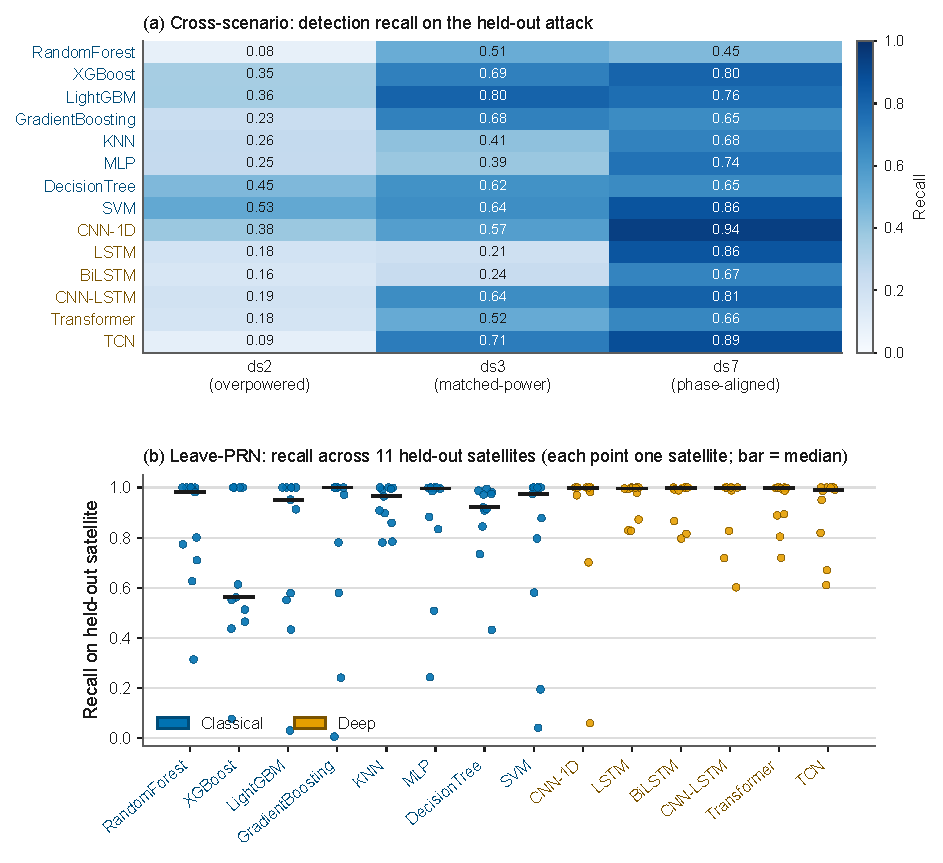
\includegraphics[width=\textwidth]{figures/fig08_generalization.pdf}
\caption{Detection recall on data held out from training. Panel (a) holds out a whole attack scenario and panel (b) holds out satellites one at a time. Recall falls in both, so the detectors depend on conditions present in their training data.}
\label{fig:generalization}
\end{figure*}

\subsection{Implications for receiver integrity}

The transmitter settings evaluated here were selected without reference to any detector,
and 126 of them capture a receiver. Approximately two fifths of those evade the strongest
detector tested, and none of that required knowledge of the detector, access to its
gradients, or the ability to query it. An adversary possessing any of those capabilities
would be strictly stronger.

For a receiver integrity monitor the practical consequence is that detection quality
measured on a fixed corpus is not a security property. It characterises behaviour on that
corpus, and a detector intended to resist an adversary must be characterised against
signals the adversary can select and emit, with the false alarm rate reported alongside.

The false alarm rates observed here carry a further implication independent of any
adversary. At a recall floor of 0.95 they span 0.337 to 0.960, so no detector in this study
is usable as a standalone single epoch integrity monitor even in the absence of an attacker.
A deployed monitor would necessarily combine decisions across epochs and across satellites,
trading detection latency against alarm rate, and the per epoch quantities reported here
are the inputs to such a scheme and not a substitute for it.

\subsection{Scope and limitations}

The adversary is restricted in the four respects set out in Section~\ref{sec:threat}, and
each restriction reduces its capability, so the failure rates reported are a lower bound on
what an unrestricted adversary could achieve. The power condition illustrates the point.
Requiring the counterfeit to exceed the authentic signal follows the established account
of capture, and it is one of the two conditions, with the code being dragged, that select
126 of the 209 swept settings as operative. Capture at lower power has since been reported by other means
\citep{liu2026dimas}, which would enlarge the operative subset and so enlarge the set of
transmissions a detector must withstand. Relaxing the condition could therefore only
raise the counts reported here.

The study covers one signal, GPS L1 C/A, and one stationary receiver at a surveyed
location. Whether the same detectors behave equivalently on other civil signals, or on a
moving platform whose dynamics enter the observables, is not established here. The
generator itself is not specific to GPS L1 C/A, and repeating the procedure on another
signal requires the corresponding spreading code and receiver configuration.

The navigation domain result rests on a common pull-off applied to all satellites, which a
stationary receiver absorbs into its clock estimate. An adversary seeking to displace the
reported position and not the clock would apply differing offsets across satellites,
and that case is not measured here.

One documented difference between the generated attack and the recorded one is reported in
Section~\ref{sec:validation}. The generated counterfeit is an amplitude matched replica, so
its cancellation is cleaner than the recorded spoofer achieved, leaving the generated
attack marginally stronger and therefore marginally easier to detect. This bias acts
against the adversary and so does not inflate the failure rates reported.

\subsection{Directions for a defence}

The results constrain what a defence can rely upon. Architecture is not sufficient, since
both model families appear among the detectors that are evaded. Clean detection quality is
not sufficient, since the detector with the best clean performance is evaded most often.
Threshold placement is not sufficient, since resistance obtained by raising the alarm rate
is paid for on authentic data.

Two directions remain open. The first is to require the detector to respect a physical
relation that authentic signals satisfy, as has been done for code carrier consistency
\citep{song2026generalized}; the library of transmitted attacks constructed here supplies
the signals against which such a detector would need to be evaluated, including the
settings that hold received power constant through Equation~\ref{eq:neutral}. The second is
to construct a detector whose behaviour under bounded input change can be certified in
advance and not estimated afterwards \citep{cohen2019certified}. Both lie outside
the scope of the present study, which characterises the behaviour of existing detectors.

\section{Conclusion}
\label{sec:conclusion}

This paper has characterised the behaviour of machine learning detectors of GNSS spoofing
under attacks that are transmitted signals selected by an adversary. Each attack was
synthesised as radio samples, summed with authentic recordings from the Texas Spoofing Test
Battery, passed through a model of the receiver front end and tracked by an open software
receiver, so that the observables each detector read were produced by receiver processing
of a transmittable waveform. The generator was validated against a recorded attack whose
construction is documented in full, and reproduced its observables satellite by satellite.

Fourteen detectors, eight classical and six deep, were placed at a common operating point
defined by a recall floor of 0.95 on clean validation data, and evaluated against 126
transmitter settings satisfying the published conditions for receiver takeover.

Clean detection performance was found to be a poor predictor of resistance. The random
forest attained the highest clean $F_1$ score at 0.833 and the lowest false alarm rate at
0.337, and failed to flag 55 of the 126 attacks, flagging 0.1 percent of the spoofed
samples of one of them. Across the set, the four detectors with the highest clean $F_1$
were evaded at 0.226 of their detector-attack pairs against 0.106 for the remaining ten,
significant at $p = 2.8 \times 10^{-10}$, although the monotone rank correlation across all
fourteen is not significant and is reported as such. The
five detectors that flagged every attack did so while flagging between 46 and 74 percent of
authentic samples, a regime in which the resistance is not operationally available. Across
all fourteen detectors, false alarm rates at this operating point ranged from 0.337 to
0.960.

One evaded attack was propagated through the navigation stage. It drove the receiver clock
at 48.89 nanoseconds per second against a commanded 48.87, while the detector with the best
clean performance classified 98.8 percent of its samples as authentic, establishing
detection failure and navigation domain effect on the same attack and the same recording.

The adversary producing these results had no knowledge of the deployed detector, computed
no gradient and issued no query, and was further restricted to a single signal, full
satellite coverage and a stationary victim. Each restriction reduces its capability, so the
reported failure rates constitute a lower bound.

The broader implication is that detection accuracy measured on a fixed corpus of recorded
attacks characterises that corpus. A detector intended to withstand an adversary requires
characterisation against signals the adversary can select and emit, reported jointly with
the false alarm rate incurred. The library of transmitted attacks constructed here is
available for that purpose, and extends directly to the evaluation of physics constrained
and certified detectors.


\backmatter

\section*{List of abbreviations}
\begin{description}
\item[CNN] convolutional neural network
\item[C/N$_0$] carrier-to-noise density ratio
\item[DLL] delay-lock loop
\item[FGI] Finnish Geospatial Research Institute
\item[FLL] frequency-lock loop
\item[GNSS] Global Navigation Satellite System
\item[GPS] Global Positioning System
\item[LSTM] long short-term memory
\item[PLL] phase-lock loop
\item[PNT] positioning, navigation and timing
\item[PRN] pseudo-random noise
\item[TEXBAT] Texas Spoofing Test Battery
\end{description}

\section*{Declarations}

\bmhead{Ethics approval and consent to participate}
Not applicable. This study involves no human participants, human data or animal
subjects; it processes recorded radio-frequency signals from a public spoofing-attack
test benchmark.

\bmhead{Consent for publication}
Not applicable.

\bmhead{Availability of data and materials}
The derived receiver-observable corpus and the evaluation code are available from the
corresponding author on reasonable request. The raw Texas Spoofing Test Battery
recordings are distributed by the University of Texas at Austin Radionavigation
Laboratory, and the FGI-GSRx software-defined receiver is released under the GPLv3
licence.

\bmhead{Competing interests}
The authors declare that they have no competing interests.

\bmhead{Funding}
The authors received no specific funding for this work.

\bmhead{Authors' contributions}
J.S.O. conceived the study, developed the methodology, implemented the experiments,
analysed the results and wrote the manuscript. W.A.A. supervised the work and
reviewed the manuscript. A.O.A. reviewed the manuscript. All authors read and
approved the final manuscript.

\bmhead{Acknowledgements}
We thank the University of Texas at Austin Radionavigation Laboratory for the Texas
Spoofing Test Battery recordings and the Finnish Geospatial Research Institute for
the open-source FGI-GSRx software-defined receiver used in this study.

\bibliography{references}

\end{document}
